\documentclass[12pt,a4paper]{report}
\usepackage{color}

\usepackage[utf8]{inputenc} % pentru suport diacritice
\usepackage[romanian]{babel} % setări pentru limba română 
\renewcommand\familydefault{\sfdefault} % sans serif

\usepackage[margin=2.54cm]{geometry}	% dimensiuni pagină și margini
\usepackage{graphicx} % support the \includegraphics command and options


\usepackage{algorithm}
\usepackage{listings}
\usepackage{adjustbox}
\usepackage{algpseudocode}


\definecolor{dkgreen}{rgb}{0,0.6,0}
\definecolor{gray}{rgb}{0.5,0.5,0.5}
\definecolor{mauve}{rgb}{0.58,0,0.82}

\lstset{frame=tb,
  language=Java,
	float=H,
  aboveskip=3mm,
  belowskip=3mm,
  showstringspaces=false,
  columns=flexible,
  basicstyle={\small\ttfamily},
  numbers=left,
  numberstyle=\tiny\color{gray},
  keywordstyle=\color{blue},
  commentstyle=\color{dkgreen},
  stringstyle=\color{mauve},
  breaklines=true,
  breakatwhitespace=true,
	stepnumber=1,
  tabsize=3
}
% formatting sections and subsections
\usepackage{textcase}
\usepackage{titlesec}
\titleformat{\chapter}{%
\large%
\bfseries%
%\MakeUppercase
}{\thechapter}{2ex}{\MakeUppercase}[\vspace*{-1.5cm}]
\titleformat*{\section}{\large\bfseries}
\titleformat*{\subsection}{\large\bfseries}
\titleformat*{\subsubsection}{\large\bfseries}

\usepackage{chngcntr}
\counterwithout{figure}{chapter} % no chapter number in figure labels
\counterwithout{table}{chapter} % no chapter number in table labels
\counterwithout{equation}{chapter} % no chapter number in equation labels

\usepackage{booktabs} % for much better looking tables
\usepackage{url} % Useful for inserting web links nicely
\usepackage[bookmarks,unicode,hidelinks]{hyperref}

\usepackage{array} % for better arrays (eg matrices) in maths
\usepackage{paralist} % very flexible & customisable lists (eg. enumerate/itemize, etc.)
\usepackage{verbatim} % adds environment for commenting out blocks of text & for better verbatim
\usepackage{subfig} % make it possible to include more than one captioned figure/table in a single float
\usepackage{enumitem}
\setlist{noitemsep}

%%% HEADERS & FOOTERS
\usepackage{fancyhdr}
\pagestyle{empty}
\renewcommand{\headrulewidth}{0pt}
\renewcommand{\footrulewidth}{0pt}
\lhead{}\chead{}\rhead{}
\lfoot{}\cfoot{\thepage}\rfoot{}

\newcommand{\HeaderLineSpace}{-0.5cm}
\newcommand{\UniTextRO}{UNIVERSITATEA POLITEHNICA DIN BUCUREȘTI \\[\HeaderLineSpace] 
FACULTATEA DE AUTOMATICĂ ȘI CALCULATOARE \\[\HeaderLineSpace]
DEPARTAMENTUL CALCULATOARE\\}
\newcommand{\DiplomaRO}{PROIECT DE DIPLOMĂ}
\newcommand{\AdvisorRO}{Coordonator științific:}
\newcommand{\BucRO}{BUCUREȘTI}

\newcommand{\UniTextEN}{UNIVERSITY POLITEHNICA OF BUCHAREST \\[\HeaderLineSpace]
FACULTY OF AUTOMATIC CONTROL AND COMPUTERS \\[\HeaderLineSpace]
COMPUTER SCIENCE DEPARTMENT\\}
\newcommand{\DiplomaEN}{DIPLOMA PROJECT}
\newcommand{\AdvisorEN}{Thesis advisor:}
\newcommand{\BucEN}{BUCHAREST}

\newcommand{\frontPage}[6]{
\begin{titlepage}
\begin{center}
{\Large #1}  % header (university, faculty, department)
\vspace{50pt}
\begin{tabular}{p{6cm}p{4cm}}

\includegraphics[scale=0.8]{pics/upb-logo.jpg} &
	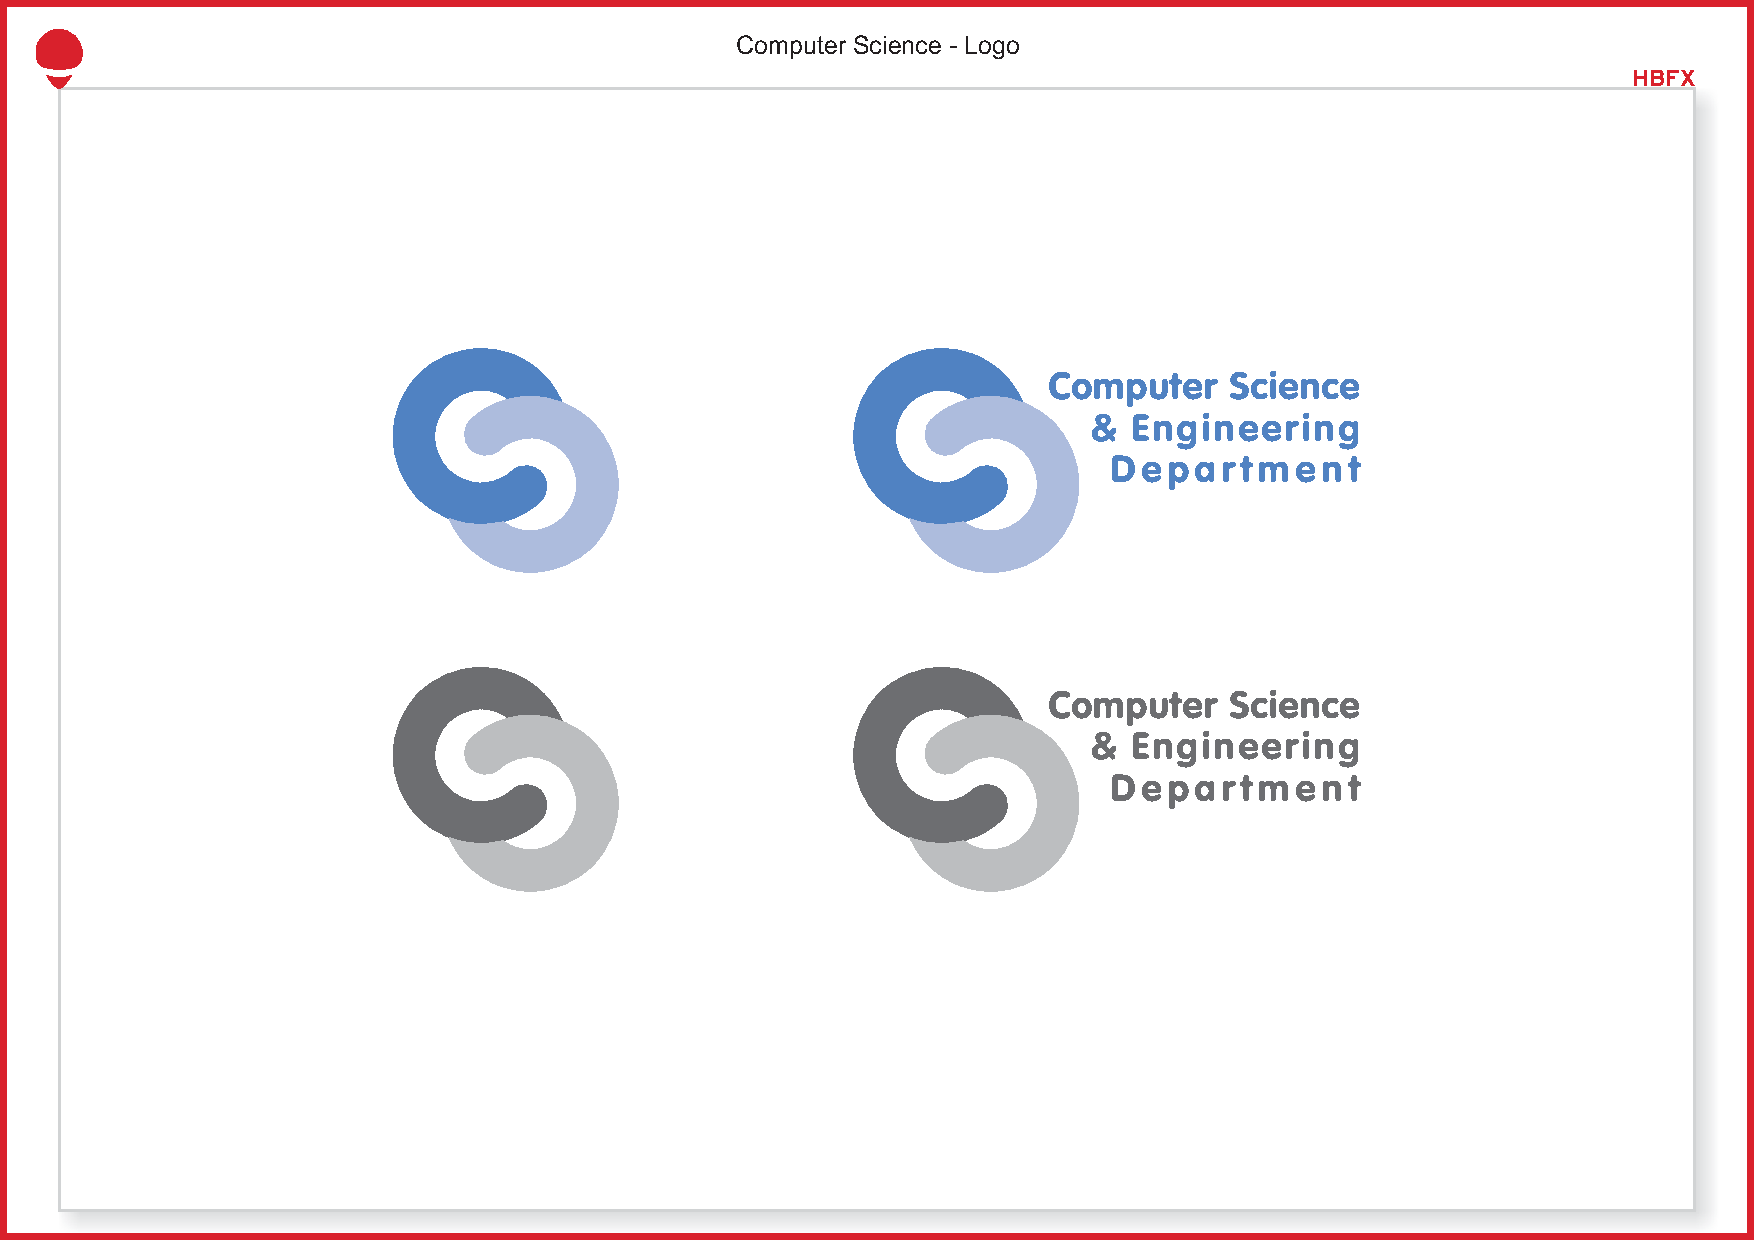
\includegraphics[scale=0.5,trim={14cm 11cm 2cm 5cm},clip=true]{pics/cs-logo.pdf}
\end{tabular}

\vspace{105pt}
{\Huge #2}\\                           % diploma project text
\vspace{40pt}
{\Large #3}\\ \vspace{0pt}  % project title
{\Large #4}\\                          % project subtitle
\vspace{40pt}
{\LARGE \Name}\\                   % student name
\end{center}
\vspace{60pt}
\begin{tabular*}{\textwidth}{@{\extracolsep{\fill}}p{6cm}r}
&{\large\textbf{#5}}\vspace{10pt}\\      % scientific advisor
&{\large \Advisor}                                    % advisor name
\end{tabular*}
\vspace{20pt}
\begin{center}
{\large\textbf{#6}}\\                                % bucharest
\vspace{0pt}
{\normalsize \Year}
\end{center}
\end{titlepage}
}

\newcommand{\frontPageRO}{\frontPage{\UniTextRO}{\DiplomaRO}{\ProjectTitleRO}{\ProjectSubtitleRO}{\AdvisorRO}{\BucRO}}
\newcommand{\frontPageEN}{\frontPage{\UniTextEN}{\DiplomaEN}{\ProjectTitleEN}{\ProjectSubtitleEN}{\AdvisorEN}{\BucEN}}

\linespread{1.5}
\setlength\parindent{0pt}
\setlength\parskip{.28cm}

%% Abstract macro
\newcommand{\AbstractPage}{
\begin{titlepage}
\textbf{\large SINOPSIS}\par
\AbstractRO\par\vfill
\textbf{\large ABSTRACT}\par
\AbstractEN \vfill
\end{titlepage}
}

%% Thank you macro
\newcommand{\ThanksPage}{
\begin{titlepage}
{\noindent \large\textbf{MULȚUMIRI}}\\
\Thanks
\end{titlepage}
}



%%%%%%%%%%%%%%%%%%%%%%%%%%%%%%%%%%%%%%%%%%%%%%%%%%   
%%
%%          End of template definitions
%%   
%%%%%%%%%%%%%%%%%%%%%%%%%%%%%%%%%%%%%%%%%%%%%%%%%%


%%% Puteți elimina aceste linii din lucrare, servesc numai pentru template.
\newcommand{\worktype}[1]{[\textit{#1}] }
\newcommand{\dezvoltare}{\worktype{Dezvoltare de produs}}
\newcommand{\cercetare}{\worktype{Cercetare}}
\newcommand{\ambele}{\worktype{Ambele}}
%%%


%%
%%   Campurile de mai jos trebuie modificate de autor. Modificati doar continutul, nu si numele fiecarei definitii
%%
\newcommand{\ProjectTitleRO}{Consistenta datelor in rețele mobile colaborative ad-hoc bazate pe paradigma Drop Computing}
\newcommand{\ProjectSubtitleRO}{version}
\newcommand{\ProjectTitleEN}{Data consistency in Drop Computing paradigm: ad-hoc dynamic collaborative computing}
\newcommand{\ProjectSubtitleEN}{version}
\newcommand{\Name}{Tăbușcă Vlăduț-Constantin}
\newcommand{\Advisor}{Șl.dr.ing. Ciobanu Radu-Ioan}
\newcommand{\Year}{2018}

% Setări document
\title{Proiect de diplomă}
\author{\Name}
\date{\Year}

%%
%%   Campurile aferente rezumatului
%%
\newcommand{\AbstractRO}{Sinopsisul proiectului are rol de introducere, conținând atât o descriere pe scurt a problemei abordate cât și o enumerare sumară a rezultatelor și a concluziilor. Se recomandă ca sinopsisul să fie redactat într-un limbaj accesibil unei persoane nefamiliarizate cu domeniul, dar în același timp destul de specific pentru a oferi rapid o vedere de ansamblu asupra proiectului prezentat.
Sinopsisul proiectului va fi redactat atât în română cât și în engleză. Ca dimensiunea recomandată aceasta secțiune va avea maxim 200 de cuvinte pentru fiecare variantă. Împreună, ambele variante se vor încadra într-o singură pagină.}

\newcommand{\AbstractEN}{The abstract has an introductory role and should engulf both a brief description of the issue at hand, as well as an overview of the obtained results and conclusions. The abstract should be formulated such that even somebody that is unfamiliar with the projects’ domain can grasp the objectives of the thesis while, at the same time, retaining a specificity level offering a bird’s eye view of the project.
The projects’ abstract will be elaborated in both Romanian and English. The recommended size for this section is limited to 200 words for each version. Together, both versions will fit in one page.}

%%
%%   Campurile aferente paginii de multumiri
%%
\newcommand{\Thanks}{(opțional) Aici puteți introduce o secțiunea specială de mulțumiri / acknowledgments. }

\begin{document}

\frontPageRO
\frontPageEN

\begingroup
\linespread{1}
\tableofcontents
\endgroup

\AbstractPage

% poate fi comentata sau stearsa
\ThanksPage


% Textul licentei incepe de aici 
\chapter{Introducere}\pagestyle{fancy}
\section{Context}
Rețelele mobile și sistemul cloud sunt printre cele mai folosite resurse de comunicare din zilele noastre, datorită dorinței de a accesa permanent și de pe orice dispozitiv informația. Această lucrare se bazează pe un nou concept, intitulat Drop computing, din cadrul rețelelor oportuniste. Această paradigmă oferă o alternativă pentru evitarea latențelor și costurilor ridicate ale cloud-ului prin utilizarea resurselor computaționale și a mobilității tuturor nodurilor pentru execuția și transferul cererilor unui singur nod. Fiecare nod, la rândul lui, poate primi rezolvarea unei cereri prin intermediul oricărui nod din rețea cu care intră în contact. Orice cerere computațională va purta în această lucrare denumirea de task. Astfel, un task se va propaga oportunist până la executant și apoi prin alte noduri intermediare până la proprietar. Această propagare oportunistă se referă la schimbul de task-uri realizat la întâlnirea dintre două noduri. Acest schimb este influențat de gradul de cunoaștere al nodului proprietar, de nivelul de altruism al nodului întâlnit, dar și de resurse computaționale precum baterie sau memorie. Aceste scenarii au deja rezultate deosebite în ceea ce privește gradul de utilizare al cloud-ului, procentul de reducere al costului fiind mult mai mare ca procentul cu care a scăzut performanța, acest lucru este detaliat în~\cite{DC}. Toate aceste rezultate s-au bazat pe următoarea presupunere: toate rezolvările care se interschimbă în rețea sunt corecte. Coruperea informațiilor atât în mod intenționat, cât și din cauza unor factori externi (e.g senzori defectați) determină un comportament nedorit în toate exemplele de utilizare ale acestor tipuri de rețele. Soluția propusă în această lucrare intervine în acest context de corupere, foarte plauzibil în viața reală, încercând să rezolve problema consistenței datelor.

\section{Problema} 
Principala utilitate a soluției propuse este reprezentată de existența unui grad de siguranță în ceea ce privește corectitudinea informațiilor transferate între nodurile unei rețele oportuniste. În momentul în care este necesară rezolvarea unui task sau se descoperă o informație dorită la unul dintre nodurile cu care se intră în contact, trebuie să cunoașteam nivelul de încredere pe care îl atribuim acelui nod și, implicit, acelei rezolvări. Problema rezolvată este cea a consistenței datelor, a diferențierii datelor corupte de cele corecte și a generării unui grad de încredere asociat fiecărui nod prezent în rețea. Totodată, o altă problemă abordată este legată de împărțirea task-urilor în rețea, astfel încât să se reușească un acces cât mai restricționat la cloud, nodurile reușind să primească rezolvarea într-un timp util de la vecini.

\section{Obiective}
Soluția descrisă în această lucrare își propune să ofere un nivel de încredere mai ridicat în ceea ce privește informațiile transferate și acceptate într-o rețea de tipul Drop Computing. În urma acestei implementări se crește procentajul de task-uri acceptate necorupte, acesta fiind de cele mai multe ori maxim, înregistrându-se însă o latență mai ridicată la procesare și un procentaj mai mic de rezolvări dobândite cu ajutorul celorlalte noduri din rețea. Aceste evoluții sunt normale, dat fiind faptul că se realizează o selecție mai restrânsă de noduri utilizate, rezultatele task-urilor generate nu ajung să fie primite mai rapid deoarece posibilitățile de propagare a informației se diminuează, deci și șansele de a ajunge mai repede la proprietar. Soluția oferă o abordare realistă, bazată pe anumite trace-uri generate în funcție de mobilitatea și de interacțiunea dintre dispozitive mobile reale. Un alt obiectiv este legat de abordarea unor comportamente și limitări ale dispozitivelor mobile, astfel încât soluția propusă să se integreze cu succes în viața reală. Printre aceste abordări se numără și nivelul bateriei, memoria limitată sau timpul de contact scurt dintre dispozitive, aspecte ce pot accentua inconsistența datelor prin replicarea lor în noduri nepotrivite.
\section{Soluția propusă} 
În această lucrare, propunem soluții pentru asigurarea consistenței datelor în rețele mobile bazate pe Drop Computing, folosind mecanismul de rating și sistemul de așteptare al versiunilor unui task înainte de a lua o decizie cu privire la corectitudinea informațiilor. Aceste mecanisme sunt completate de diferite limitări în ceea ce privește calea parcursă de o versiune a task-ului, precum: procent diferit de executanți, o frecvență maximă a nodurilor parcurse, dar și o condiție de familiaritate ridicată între nodurile intermediare. Alături de transmiterea solitară a biților de date prin rețea, se implementează și un sistem de detecție și corecție al unor biți corupți utilizând codurile Hamming. În funcție de caracteristicile rețelei și de cantitatea de overhead permisă se simulează atât doar transmiterea datelor utile, cât și folosirea unor informații redundante alături de biții de date. Multiplele transferuri de informații care pot apărea în rețea sunt diferențiate după momentul de timp, categoria task-ului și după perechile de participanți ce interschimbă task-uri. Totodată, pentru generarea unui overhead cât mai mic, se limitează atât numărul de mesaje, cât și perioadele în care acestea se propagă în rețea alături de task-urile executate. // pentru a realiza o cunoaștere a întregii 
\section{Rezultatele obținute}
Pe baza mecanismelor de consistență propuse, arătăm prin simulări și experimente că putem îmbunătăți rata de task-uri corecte în Drop Computing cu până la 80\% în anumite situații concrete, fără să afectăm latența prea mult. Ținând cont de limitările rețelelor mobile oportuniste cu privire la nivelul scăzut de overhead permis, dar și lipsa unui sistem de administrare central, am creat statistici relevante care să măsoare atât punctele tari, cât și punctele slabe ale implementării propuse. Punctele tari sunt reprezentate de numărul ridicat de informații corecte acceptate la destinație și de identificarea corectă a nodurilor corupte. Cel mai reprezentativ rezultat fiind cel în care, în ciuda numărului majoritar de versiuni corupte, existente în acel moment în toată rețeaua, nodul destinatar acceptă o versiunea corectă. Acest rezultat reprezintă dovada evidentă a filtrării nodurilor într-adevăr corupte și a acceptării unor versiuni ce au parcurs o rută evaluată sigură în mod corect. Punctele slabe sunt identificate prin latența de procesare al unui task ce se încearcă a fi rezolvat cu ajutorul nodurilor întâlnite. Acest dezavantaj este caracteristic întregului concept de Drop Computing, însă, odată cu filtrarea anumitor noduri și cu așteptarea mai multor versiuni este normal să se accentueze deoarece se diminuează numărul de noduri cu care se interschimbă informații. Provocarea implementării acestui mecanism de așteptare este de a păstra în continuare un procentaj ridicat de task-uri executate de nodurile rețelei și distribuite către beneficiar într-un timp specific fiecărei rețele. 

\section{Structura lucrării}
Lucrarea se deschide cu capitolul~\ref{motivatie}, acesta sintetizează numeroase utilități ale paradigmei de Drop Computing oferind și 3 exemple concrete din viața reală. În continuare, capitolul~\ref{metodeExistente} descrie paradigmele din care a evoluat Drop Computing, iar în final se analizează mecanismele de replicare a informațiilor prezentate în diverse lucrări de la diferite conferințe de specialitate. Descrierea mecanismelor de realizare a consistenței este împărțită între capitolele~\ref{solutiaPropusa} și~\ref{detalii}. Primul, din cele două menționate, descrie o abordare teoretică în funcție de nevoile rețelei, în timp ce al doilea capitol detaliază necesitatea unor raționamente prin prezentarea unor scheme grafice, la care se adaugă și descrierea unor algoritmi sugestivi în pseudocod. Capitolul~\ref{evaluare} prezintă un set de grafice care analizează, pe diferite scenarii de corupere și de realizare a consistenței, 3 metrici care sunt dezbătute la început de capitol.
Capitolul~\ref{concluzii} sumarizează implementarea întregului proiect și analizează rezultatele obținute dezbătând atât punctele tari, cât și limitările pe care acestea le sugerează. În final, capitolul~\ref{bibliografie} este format din toate intrările bibliografice ce au fost citate în aceată lucrare. Pentru o mai bună înțelegere, a unor aspecte ce vor fi descrise în continuare, se vor face trimiteri la fragmente de cod, grafice și informații optionale ce au fost adăugate în capitolul Anexe. 


\chapter{Motivație} \label{motivatie}

Aplicațiile mobile de astăzi oferă funcționalități din ce în ce mai ample și mai inovatoare pentru utilizatorii finali. În ciuda resurselor de calcul impresionante ale unui telefon inteligent, toate aceste aplicații se bazează pe suportul cloud-ului pentru a oferi utilizatorului cea mai bună interacțiune. Din cauza numeroaselor interacțiuni cu cloud-ul apar anumite limitări și provocări în ceea ce privește nivelul de încărcare al rețelei, întrucât chiar și pentru o conexiune între două dispozitive aflate în aceeași proximitate se așteaptă răspuns de la cloud.

\section{Rețele mobile și Drop Computing}
Interacțiunea cu un sistem cloud este benefică și necesară pentru dispozitive cu o putere locală de calcul limitată, dar și costisitoare atât ca infrastructură, cât și ca timp de așteptare al răspunsurilor. Pentru a restrânge această interacțiune, trebuie limitată cantitatea de date trimise către platformele cloud prin mutarea unor părți de prelucrare a datelor la marginea rețelei, mult mai aproape de unde au fost generate informațiile. În cadrul unei rețele formate din dispozitive mobile, pentru a avea acces la date sau putere de calcul, un dispozitiv (denumit în continuare nod) va face o cerere către anumite servere din cloud. Pentru a evita latențele ridicate ale cloud-ului, dar și costurile importante de găzduire, există așa numita paradigmă de "Edge Computing". Această paradigmă se referă la existența anumitor routere, switch-uri sau set-top-box-uri, în aceeași rețea cu dispozitivele mobile, ce pot să facă caching la datele primite de la Cloud sau care pot chiar resolva task-uri, fără a mai fi nevoie să se trimită request-uri în cloud. Astfel, atunci când un dispozitiv necesită folosirea anumitor date sau calcule computațional intensive, întreabă mai întâi nodurile edge dacă au datele sau pot rezolva task-urile respective, iar în caz afirmativ datele vor fi preluate de la acestea fără a mai realiza conexiunea cu sistemul cloud.

Extinzând modelul de "Edge Computing", pentru a îmbunătăți și mai bine atât latența, cât și costurile, ceea ce fac dispozitivele edge, pot la fel de bine să facă și nodurile mobile. Astfel, paradigma Drop Computing sugerează ca fiecare nod mobil să poată face caching pentru datele și rezultatele provenite din cloud, ce pot fi necesare și valorificate de alte noduri. Alături de date provenite direct de la cloud, fiecare nod poate reține în memoria locală, atât informațiile complete calculate de alt vecin, cât și task-urile de rezolvat ale nodurilor cu care a intrat în contact. Toată această multiplicare a informațiilor în rețea va ajuta la un timp de răspuns mult mai bun atunci când o informație va fi cerută de celelalte noduri mobile din rețea. Totodată, datorită mobilității nodurilor, datele propagate oportunist pot ajunge de la destinatar către expeditor și în situația când nu există o legătură directă între aceștia, nefiind conectați la Internet. Rezultatele obținute din această abordare au sugerat o importantă aplicabilitate în viața reală, identificându-se un impact major în scăderea încărcării unei platforme cloud, în timp ce interacțiunea utilizatorului cu dispozitivul mobil nu a fost afectată sesizabil în materie de timp de așteptare~\cite{DC}.

\section{Cazuri de utilizare}
Motivația realizării acestei lucrări este evidețiată de multiple scenarii din viața reală ale căror desfășurare este influențată prin mecanismele de aducere a datelor și a resurselor computaționale mai aproape de utilizatorul final. În continuare, vom prezenta câteva scenarii uzuale ce vor beneficia de existența unui sistem complet care implementează caracteristicile paradigmelor introduse în această secțiune. Un prim exemplu presupune mulțimi de oameni adunați cu un scop comun, cum ar fi vizionarea unui important meci de fotbal pe un stadion cu un număr impresionant de locuri. Presupunând că majoritatea participanților dețin un telefon mobil, dacă jumătate au nevoie să utilizeze conexiunea 3G/4G/Wi-Fi în același moment de timp, serviciul oferit va fi unul fragmentat ce va conduce la o interacțiune neplăcută. Chiar dacă stadionul oferă semnal Wi-Fi în mai multe puncte, conectarea unui număr de ordinul miilor la același access point duce la o împărțire foarte intensă a lungimii de bandă, având ca rezultat o conexiune foarte lentă. Ținând cont de faptul că o asemenea mulțime ar putea fi interesată de lucruri similare accesate pe Internet, precum aflarea rezultatului la un alt meci sau programul mijloacelor de transport în comun, o paradigmă precum Drop Computing are o puternică utilitate. Astfel, în schimbul conexiunilor cu access point-urile din stadion sau stațiile GSM din aria respectivă, dispozitivele se pot conecta între ele până când se întâlnește un nod cu informația căutată. Un nod mobil poate deține informația fie printr-o descărcare directă folosind 3G/4G/Wi-Fi, fie printr-o salvare a informațiilor primite de la nodurile întâlnite. Acest exemplu identifică rețelele oportuniste ca o alternativă viabilă pentru soluții precum Wi-Fi,GSM în momentul în care infrastructura acestora nu poate rezolva un număr mare de cereri, sau nu funcționează corect în anumite porțiuni.
% un paragraf cam mare?

Un alt scenariu de folosire potrivită a paradigmei Drop Computing este reprezentat de implementarea aplicațiilor mobile CPU-intensive. De exemplu, o aplicație de editare fotografii prezintă o serie de operații complexe care, pe măsură ce numărul utilizatorilor crește, necesită o infrastructură cloud puternică pentru partea de backend. Pentru o bună interacțiune a utilizatorilor, indiferent de puterea de calcul a dispozitivului ce rulează aplicația, menținerea unei platforme cloud puternice necesită atât costuri ridicate, cât și multă muncă din partea dezvoltatorilor. În această situație, folosind rețele de vecini formate și aflate într-o continuă schimbare în jurul dispozitivului mobil pentru distribuirea calculelor computațional intensive, rezultă o mai bună interacțiune a utilizatorului cu aplicația. Datorită comunicării cu dispozitivele întâlnite și utilizarea lor pentru a aduce date de la cloud sau pentru a realiza calcule mai rapid, se reduce latența cererilor și răspunsurilor frecvente către sau dinspre cloud.
% tot aici exemplu cu realizari militare

Una dintre cele mai importante situații reale în care folosirea rețelelor mobile oportuniste de la baza unei infrastructuri de tip Drop Computing, reprezintă un beneficiu important este reprezentată de organizarea în cadrul unor calamități naturale. În multe situații de criză, în urma unor dezastre naturale sau a altor împrejurări care determină prăbușirea unor elemente de infrastructură (stâlpuri căzute, cabluri rupte, switch-uri distruse), atât comunicarea între membrii echipajului de salvare, cât și comunicarea cu victimele implicate este crucială. În prezent, oamenii cel mai adesea comunică folosind dispozitive mobile inteligente, trimițând informații despre starea lor către cei dragi prin intermediul aplicațiilor ce necesită acces la Internet. O actuală soluție se bazează pe folosirea rețelelor oportuniste, astfel creându-se o nouă infrastructură suprapusă peste cea distrusă, în care componentele neafectate se comportă precum nodurile mobile dintr-o rețea oportunistă. Având ca scop realizarea unei conexiuni neîntrerupe, folosirea oricărui dispozitiv mobil al unei victime sau al persoanelor aflate în regiunea restrânsă în care s-a produs dezastrul crește șansele de a găsi cât mai repede persoanele care au nevoie de ajutor. Ținând cont de faptul că modelul de mobilitate al nodurilor în cazul unor astfel de evenimente este mult mai predictibil (persoanele posesoare de dispozitive deplansându-se către zonele de refugiu din apropiere), împărțirea datelor în rețea se poate face mult mai eficient ținând cont în special de nodurile care rămân blocate și ale căror date devin obligatoriu de transferat. Astfel, informații obligatorii precum poziția geografică a nodului sunt purtate oportunist și reușesc să ajungă la echipajul de salvare mult mai repede, în momente în care timpul poate însemna viața. Aceste aplicații trebuie să fie prezente întotdeauna pe dispozitivele mobile, iar scenariile privind infrastructura să fie simulate periodic atât pentru a se familiariza utilizatorii cu folosirea lor, cât și pentru a testa transmiterea de date. Datele corecte sunt cele mai importante, iar orice informație recepționată cu o valoare eronată poate avea consecințe nefericite în cadrul unei situații de urgență.

\section{Necesitate}
Din ceea ce am prezentat în paragrafele anterioare, atât în lucrarea Drop Computing~\cite{DC}, cât și în alte lucrări din literatura de specialitate, este identificată problema consistenței datelor în momentul în care informații sau task-uri sunt împrăștiate prin rețea. Acest lucru conduce la următoarea întrebare: cum știe un nod că datele de care are nevoie, pe care i le oferă alt nod mobil, sunt corecte, nefiind corupte sau modificate intenționat de niciun nod care le-a deținut la un moment dat? Această necesitate științifică exprimată în domeniul rețelelor mobile este principala motivație pentru această lucrare de licență. Așadar, pentru a evita situația folosirii de date corupte, vom prezenta anumite mecanisme de realizare a consistenței datelor alături de posibilitatea ca un nod mobil să sesize primirea unor date corupte. În același timp, există necesitatea de a cunoaște un mod de împărțire a datelor pe nodurile rețelei astfel încât să se păstreze consistența și, totodată, rețeaua să fie acoperită cât mai bine pentru a nu fi nevoie de request-uri frecvente către cloud sau nodurile edge.

Concluzionând, este foarte important ca tot acest mecanism de caching și împărțire a datelor realizat de toate nodurile mobile din rețeaua creată să poată oferi un anumit grad de siguranță în ceea ce privește posibilitatea primirii unor informații corupte de la nodurile cu care se intră în contact. Fiecare nod trebuie să aibă posibilitatea să recunoască date corupte și neconsistente și prin diseminarea acestor informații, să ajungă la un nivel ridicat de cunoaștere a gradului de încredere în fiecare nod din rețea. Astfel, cu ajutorul unor mecanisme ce urmează a fi prezentate în această lucrare, considerăm că se rezolvă o problemă identificată în cadrul rețelelor formate în majoritate din dispozitive mobile, fără a folosi anumite presupuneri ce nu se pot regăsi niciodată în viața reală (precum mobilitate scăzută, timp constant de contact, sau o memorie nelimitată a nodurilor implicate).

\chapter{Metode Existente} \label{metodeExistente}
În cadrul acestui capitol vom prezenta diferite tipuri de rețele mobile care, ulterior, au ajutat la crearea detaliilor paradigmei Drop Computing. Principale metode de consistență existente, discutate în diverse lucrări ce vizează aceste tipuri de rețele, fac referire la mecanisme de replicare a datelor în privința aduceri unei valori consistente cât mai aproape de beneficiar. Așadar, vom prezenta atât soluțiile, cât și problemele dezbătute în cadrul acestor abordări, ulterior, prezentând și perspectiva acestei lucrări cu privire la posibilitatea coruperii intenționate a datelor.
Secțiunea~\ref{reteleOportuniste} conține descrierea principalului tip de rețele care au stat la baza ulterioarelor dezvoltări către Drop Computing. Următoarea secțiune,~\ref{mobileEdgeComputing}, descrie următorul pas în evoluția rețelelor oportuniste, iar secțiunea~\ref{dropComputing} descrie paradigma ce stă la baza acestei lucrări. În final, secțiunea~\ref{metodeExistenteConsistenta} detaliază principalele mecanisme de realizare a consistenței în cadrul acestor rețele, aducând în discuție numeroasele presupuneri pe care se bazează soluțiile existente.  
 
\iffalse 
\section{Mobile Ad Hoc Networks(MANET)}
Foarte mulți cercetători și-au reorientat atenția și studiul în domeniul rețelelor, astfel că, pe lângă studiul intens legat de rețelele centralizate, precum Internetul și rețelele celulare, aceștia s-au orientat către studiul rețelelor descentralizate fără fir. Este vorba despre așa numitele rețele ad-hoc\cite{MITArticle}. Acestea sunt rețele formate pe loc, la nevoie, și nu necesită existența unei infrastructuri solide și complexe, așa cum presupune Internetul, putând avea aplicații în detecția distribuită, robotică, posibil chiar și în comunicațiile personale.

Principala diferență dintre aceste rețele este reprezentată de faptul că în cadrul Internetului toată responsabilitatea direcționării traficului de date aparține unor dispozitive speciale, denumite routere, acestea fiind programate în privința împărțirii pachetelor, cu toate formele de filtrare pe care ni le dorim. În schimb, în cadrul rețelelor ad-hoc, nu există stații de bază și nu există dispozitive care să monitorizeze performanța rețelelor ca un intreg. O trăsătură importantă a tuturor rețelelor ad-hoc este aceea că au loc schimbări constante în topologia rețelei, acest lucru devenind o problemă din cauza faptului că dispozitivele mobile au o autonomie cât se poate de limitată. Participanții din cadrul unor astfel de rețele nu pot transmite orice cantitate de date pentru a se acomoda cu schimbările de topologie, indiferent de distanța care îi separă.

Pentru aceste rețele schimbul de fișiere sau de date joacă un rol important care implică mulți utilizatori. Pentru a facilita împărțirea datelor se folosește ideea de replicare a datelor\cite{CDRA}, dar considerentele de care trebuie ținut seama în aceste rețele complică acești algoritmi de replicare. Frecventele partiționări ale rețelei din cauza mobilității nodurilor sau puterea limitată a bateriei conduc la o reducere a disponibilității datelor în rețea. De aceea, un algoritm eficient de replicare trebuie să găsească soluții pentru toate aceste limitări ale rețelei. Așadar, problemele de care trebuie ținut cont sunt următoarele:
\begin{itemize}
	\item\textbf{Consumul de putere} \hfill \\
	Dacă unui nod cu o baterie redusă îi sunt replicate multe bucăți de date, după puțin timp el se va opri și nu va mai putea oferi niciun serviciu. De aceea, trebuie verificat periodic nivelul de putere al fiecărui nod și datele trebuie să fie replicate doar în cele cu suficientă putere.
	\item\textbf{Mobilitatea nodurilor} \hfill \\
	Algoritmul de replicare trebuie să suporte o predicție a mobilității și, astfel, dacă un nod e posibil să părăsească rețeaua (să ajungă la o distanță neaccesibilă), datele stocate pe acest nod trebuie să fie transferate pe un alt nod a cărei predicție sugerează că se va afla cel puțin un anumit timp in rețea.
	\item\textbf{Timpul de răspuns} \hfill \\
	Timpul este un factor crucial pentru multe aplicații și, de aceea, trebuie avut în vedere ca accesul la o data cerută să fie făcut de la cel mai apropiat nod care o deține.
	\item\textbf{Mecanism de consistență} \hfill \\
	Dacă o data este read-only performanța poate fi îmbunătățită prin replicarea datei în toate nodurile (aici intervenind însă resursele limitate ale rețelei). Însă, dacă o dată este și modificată în mod frecvent, alte replici devin invalide, fiind necesar un mecanism care să verifice și să mențină consistența datelor în rețea.
\end{itemize}
Din ce am prezentat până acum se poate observa nevoia de a evolua de la MANET la un alt tip de rețele în care să nu mai fie nevoie de stocarea informațiilor de rutare și răspândirea lor in rețea în mod frecvent, deoarece această desfășurare nu este deloc fezabilă în cadrul rețelelor foarte mari. În concluzie, rețelele mobile ad-hoc (MANET-urile) au evoluat, în mod natural, în așa numitele rețele oportuniste, a căror prezentare o voi face în secțiunea următoare.
\fi

\section{Rețele oportuniste} \label{reteleOportuniste}
Principala încadrare a acestui tip de rețele se poate oferi spunând că sunt un tip de rețele tolerante la întârzieri (Delay Tolerant Networks) și, totodată, o extensie a rețelelor mobile ad-hoc (MANET). Cea mai importantă diferență față de MANET-uri o constituie faptul că rețelele oportuniste se bazează pe o mobilitate foarte ridicată a nodurilor implicate, generând între ele rute foarte dinamice. Mai mult decât atât, din cauza faptului că majoritatea conexiunilor nu sunt stabile și se întâmplă la momente de timp neregulate, de cele mai multe ori nu există o cale completă între transmițător și destinatar. Acest tip de rețele se bazează pe o paradigmă denumită store-carry-forward. Această denumire este una sugestivă întrucât un nod sursă care dorește să transmită un mesaj îl stochează local, apoi îl poartă prin rețea, urmând ca în final să îl livreze la destinație în cazul în care întâlnește nodul destinator. Dacă între proprietarul mesajului și destinatar nu se creează un contact, mesajul este transmis către un nod care prezintă mai multe șanse de a transporta mesajul la destinație sau cât mai aproape de destinație, în cel mai optim timp.

Oportunitatea se referă la faptul că un nod poate trimite un mesaj doar în momentul în care nodurile intermediare apar în suprafața de conectivitate, această suprafață depinzând de tehnologia folosită(ex. Bluetooth, Wireless, GSM). Totodată, rețelele oportuniste se bazează pe altruismul nodurilor, fiecare nod ținând cont și de interesul vecinilor de a le transporta mesajele pentru a ajunge cât mai rapid la destinație. Astfel, împărțind datele cât mai dinamic prin rețea crește probabilitatea de a ajunge la destinație, în timp ce probabilitatea ca datele să atingă nodul destinație într-un timp mult prea mare, scade. Există două tipuri de comunicare oportunistă, acestea fiind: rutare și diseminare. În timp ce primul tip presupune comunicarea cu un singur destinatar identificat cu un id unic, cel de-al doilea tip nu se mai referă la o comunicație punct-la-punct. Diseminarea se referă la faptul că nodurile pot genera date pentru o anumită categorie, în același timp ele putându-se și abona la diferite categorii de conținut de la care vor aștepta date. 
Figura~\ref{fig:pic1} sugerează o altă întrebuințare a rețelelor oportuniste dezbătută în ultimii ani și anume: \textit{data and computation offloading}.
\begin{figure}[th]
\centering
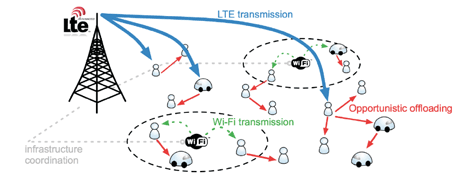
\includegraphics[width=3in]{pics/ONs.png}
  \caption{Scenariul descărcării oportuniste\protect\footnotemark}
  \label{fig:pic1}
\end{figure}
\footnotetext{© https://ercim-news.ercim.eu/en94/special/mobile-opportunistic-traffic-offloading-for-map-based-adas-applications}
Ideea de bază constă în faptul că ~\textit{offloading-ul} poate fi mult mai benefic în momentul în care un număr mare de noduri aflate în aceeași comunitate sau în comunități apropiate (fiind situate într-o arie fizică compactă), doresc să descarce aproape aceeași informație în aproximativ același timp de la serverele centrale. Așadar, fiecare nod are posibilitatea de a primi informația dorită de la un nod cu care s-a întâlnit, care la rândul lui are informația fie de la alte noduri cu care a avut contact în comunitate, fie folosim rețeaua celulară.

În literatura de specialitate întâlnim numeroși algoritmi de rutare în rețele oportuniste, fiecare având avantaje și dezavantaje în funcție de caracteristicile rețelei. Majoritatea mecanismelor de a împărți date în rețelele oportuniste se bazează pe distribuția de date Epidemic, care presupune că în momentul în care două noduri se întâlnesc primul nod își transferă toate datele la nodul întâlnit.\iffalse Acesta din urmă le salvează pe cele pe care nu le deținea deja dintr-o întâlnire anterioară și îi transferă și el propriile date. Punctele tari ale acestui mecanism sunt reprezentate de faptul că numărul mare de copii din rețea reduce întârzierea de transmitere, oferă o rată maximă mesajelor generate de a ajunge la destinație, fiind în același timp și cel mai simplu de implementat.\fi În această distribuție, punctele slabe sunt reprezentate atât de nevoia ca nodurile să aibă o memorie nelimitată, cât și de inundarea rețelei cu mesaje, ceea ce face că în această formă să fie practic imposibil de folosit în viața reală. Așadar, implementările acestei distribuții au folosit un număr limitat de mesaje pentru a putea preveni aglomerarea rețelei, dar și din cauza faptului că toate nodurile vor avea o memorie limitată. Spray and Wait~\cite{SprayAndWait} este un astfel de algoritm care, deși limitează numărul de mesaje ce pot fi trimise în rețea, păstrează o rată ridicată de reușită. Acest algoritm presupune un număr limitat și predefinit de copii pe care un mesaj al unui anumit nod le poate avea în rețea. Astfel, identificăm două faze, și anume, faza de împrăștiere și faza de așteptare. În primă fază, fiecare nod primește câte o copie a mesajului în ordinea în care sunt întâlnite, până se ating numărul de copii permise, apoi începe faza a doua, de așteptare. În această fază, nodurile ce dețin copia mesajului așteaptă întâlnirea nodul destinație, deoarece doar acestuia îl mai pot transfera. Deși această versiune nu garantează o rată maximă de reușită, valoarea ei este una ridicată ținând cont că rezolvă o problemă importantă, și anume congestia rețelei. 
\section{Mobile Edge Computing} \label{mobileEdgeComputing}
În zilele noastre, utilizatorii de dispozitive mobile inteligente sunt dependenți de execuția unor operații intensive pe acestea. Majoritatea serviciilor oferite de diverse companii, precum: Facebook, Amazon, Google, dar și conținutul de pe Youtube sau Twitter este salvat în cloud. Astfel, pentru a realiza interacțiunea dorită cu aceste aplicații informațiile cerute de utilizator trebuie descărcate local. Pentru o interacțiune cât mai plăcută, trebuie să aducem cloud-ul cât mai aproape de utilizator și de marginea rețelei, alte soluții legate de infrastructura sistemului cloud fiind mult mai scumpe și dificil de implementat. Pentru aceste cerințe ale utilizatorilor se introduce idee de Mobile Edge Computing (MEC), idee ce presupune ca resursele necesare atât stocării, calculării, cât și rețelisticii să fie integrate alături de stațiile de bază, mult mai aproape de utilizatorul final. Așadar, aplicațiile ce presupun un calcul intensiv și o latență semnificativă pot fi găzduite la marginea rețelei, datele lor fiind propagate mult mai ușor și rapid către destinatar, acest aspect fiind evidențiat și in Figura~\ref{fig:pic0}.
\begin{figure}[th]
\centering
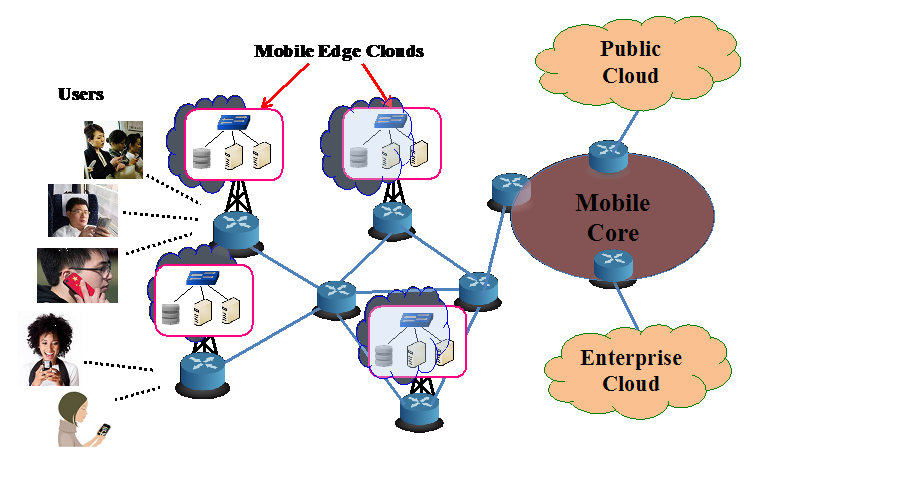
\includegraphics[width=3in]{pics/mobile-edge-computing.jpg}
  \caption{\emph{Exemplificarea cloud-urilor formate la marginea rețelei}\protect\footnotemark}
  \label{fig:pic0}
\end{figure}
\footnotetext{© https://sdn.ieee.org/newsletter/march-2016/mobile-edge-computing-an-important-ingredient-of-5g-networks}
Într-o altă paradigmă, Internet Of Things, procesarea datelor este făcută de dispozitive aflate în aceeași rețea cu mașinăriile care au generat datele, astfel cu mecanisme de caching datele de pe cloud sunt accesate cu o latență scăzută datorită faptului că ele sunt transferate mai aproape de punctul de interes grație rețelelor Content Delivery (CDNs). Mobile Edge Computing-ul\cite{MecSurvey} sugerează folosirea unei scalări a comunicației pe orizontală în detrimentul unei scalări verticale de infrastructură cloud, în momentul în care modelul de date din cloud nu mai este fezabil. Această paradigmă oferă un mediu de calcul extrem de distribuit, folosit atât pentru dezvoltarea de aplicații și servicii, cât și pentru stocarea și procesarea datelor mult mai aproape de dispozitivele mobile. O aplicație poate fi divizată în mai multe sub componente care să fie împărțite independent prin rețea. Astfel, o parte din cerințe poate ajunge să fie rezolvată fie într-un cloud format local, la marginea rețelei, fie de sistemul cloud central atât timp cât latența și precizia rămân în limitele dorite.

Așa cum reiese și din cele prezentate mai sus, conceptul de Mobile Edge Computing se concentrează pe anumite metrici importante, cum ar fi: latența și lățimea de bandă ridicată necesară comunicării. Aceste aspecte se îmbunătățesc prin limitarea transferului de date către serverele centrale, transfer ce prezintă un cost ridicat de întârziere, sprijinind astfel folosirea resurselor aflate la marginea rețelei. De asemenea, consumul de putere reprezintă o importantă grijă, prin urmare task-urile intens computaționale sunt mutate de la resursele dispozitivului utilizatorului către sisteme externe cu resurse puternice. Toate aceste îmbunătățiri vin cu un cost ridicat de implementare, deoarece atât crearea infrastructurii pentru sistemul computațional local, cât și mentenanța lui necesită un important buget. 

\section{Drop Computing} \label{dropComputing}
Paradigma de Drop Computing\cite{DC} presupune descentralizarea computing-ului peste rețele cu mai multe nivele, prin combinarea tehnologiilor cloud si wireless peste o mulțime socială formată din dispozitive mobile si de margine. Astfel, în loc ca fiecare cerere de date sau calcule să fie direcționată către cloud, Drop Computing folosește dispozitivele din proximitate pentru un acces mai rapid și mai eficient. Nevoia pentru caracteristicile aceastei paradigme vine din insuficiența modelului cloud clasic, model care deja devine nepotrivit în marea ascensiune a scenariului Internet of Things. Când un număr mare de dispozitive comunică între ele, toate sunt nevoite să trimită cereri către cloud, să aștepte răspunsul și apoi să-l proceseze, chiar dacă aceste dispozitive sunt chiar și la câțiva pași distanță unele față de altele.
Ca o concluzie, principalul scop al acestei paradigme este să minimizeze consumul de energie, să reducă costurile operaționale și chiar să mărească performanțele rețelelor mobile comparativ cu celelalte modele, atât ca timp, cât și ca nivel de siguranță.
	
\begin{figure}[th]
\centering
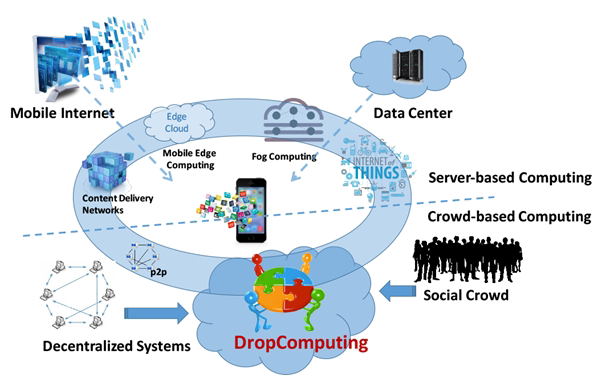
\includegraphics[width=3in]{pics/dropComputing.png}
  \caption{Viziunea Drop Computing}
  \label{fig:pic2}
\end{figure}
Așa cum sugerează și Figura~\ref{fig:pic2}\footnote{Această imagine a fost preluată din articolul\cite{DC}} de mai sus, viziunea Drop Computing este de a extinde până la extrem modelul edge cloud. Astfel, în loc de a avea dispozitive de margine fixe care să facă legătura cu cloud-ul, avem un cloud de margine. Acesta reprezentând o rețea dinamică ad-hoc formată din dispozitive mobile aflate într-un anumit perimetru. Principala noutate a acestei paradigme provine din faptul că mobilitatea nodurilor este considerată o caracteristică, o calitate și nu este văzută ca o problemă, așa cum a fost percepută până acum. Astfel, conexiunile sociale între dispozitive, mai exact între persoanele purtătoare și posesoare de dispozitive mobile, sunt utilizate pentru a calcula atât nivelul de încredere, cât și nivelul de reușită atunci când se folosesc resursele altor noduri. Concluzionând, distribuirea și salvarea datelor de către nodurile din rețea care au o probabilitate mare de întâlnire cu dispozitivele ce necesită acele informații, reprezintă un important beneficiu datorită faptului că datele sunt aduse mult mai aproape de utilizator, interacțiunea cu cloud-ul nemaifiind atât de intensă.

\iffalse
\section{MobEmu}
MobEmu~\cite{MobEmuArticle} este un simulator de rețele oportuniste care poate repeta un comportament, un trace care este fie rezultatul unei măsurători din viața reală, fie este rezultat în urma rulării unui model sintetic de mobilitate. Pe aceste rezultate putându-se aplica orice algoritm de rutare și diseminare creat de utilizator.
În timp ce modelul fizic presupune analiza unui experiment în care participanții poartă diferite dispozitive care înregistrează interacțiunile dintre ei, ca moment de timp și durata contactului, modelele sintetice sunt modele matematice ce pot simula diferite comportamente ale nodurilor. Dacă modelul Shortest Path Map-Based~\cite{ShortestPathMapBased} alege viteza de deplasare a nodurilor în mod aleator, următoarea poziție o alege aleator dintr-o listă de puncte valide, calculate de pe hartă. În continuare, acest model utilizează un algoritm de calcul pentru cel mai scurt drum dintre două puncte, precum Dijkstra, găsind cel mai scurt drum până la destinație, în funcție și de anumite direcții valide (e.g care să nu treacă prin ziduri). 

Pentru a putea rula și testa soluțiile care au stat la baza acestei lucrări am folosit MobEmu, un simulator scris in Java a cărui funcționalitate o voi descrie in continuare. În primul rând, acest framework oferă posibilitatea alegerii între mai multe tipuri de parsere: de la cele care simulează modelele sintetice, până la cele care analizează datele reale colectate de diferite dispozitive aflate în contact. La fiecare moment de timp, de când s-a măsurat trace-ul și până când s-a terminat, se verifică orice contact care apare între oricare două noduri. În momentul în care a avut loc un contact se poate folosi orice algoritm de rutare și diseminare preferat și implementat de utilizator. 
În al doilea rând, MobEmu permite ca utilizatorul să controleze la fiecare moment de timp generarea de mesaje a unui nod către alte noduri, dar și numărul lor, prioritatea, Time-To-Live, numărul total de copii pe care le permite în rețea. Totodată, simulatorul calculează comunitatea din care face parte fiecare nod utilizând algoritmul k-CLIQUE sau alți algoritmi care utilizează detecția bazată pe euristici cognitive. 

În final se oferă statistici cu privire la numărul de mesaje care au ajuns la destinație, timpul în care acestea s-au propagat prin rețea, numărul de comunități create, latența și costul transportului. Toate aceste informații fiind influențate de anumite setări pe care le poate face utilizatorul, precum memoria fiecărui nod, viteza cu care mesajele se pot transmite, dar și nivelul de altruism al nodurilor.
Pe lângă acest simulator, mai există și altele care se comportă în mod asemănator, cel mai cunoscut fiind ONE (Opportunistic Network Environment)~\cite{OneArticle} disponibil tot in Java și care modelează mobilitatea nodurilor, contactele inter noduri, dar și rutarea pachetelor. În cadrul lui, fiecare nod este reprezentat de un modul principal care la rândul lui se poate conecta la diferite submodule precum: energia consumată, mobilitatea, memoria, descriind astfel capabilitățile și atributele nodului ONE. Decizia de a folosi MobEmu a venit în urma unor avantaje pe care acesta le oferă, și anume: suport pentru detectarea comunităților de noduri, folosirea conexiunilor din rețelele sociale, modelarea altruismului, permițând în același timp și simularea unor comportamente în care mesajele nu sunt propagate către o singură destinație. Aceste avantaje am considerat că se mapează mult mai bine pe situațiile reale, în care posesorii dispozitivelor inteligente pot respecta un anumit tipar de mobilitate sau de conținut accesat, atât datorită relațiilor sociale generale, cât și datorită comunității din care fac parte in acel moment.  
\fi

\section{Metode de realizare a consistenței datelor} \label{metodeExistenteConsistenta}
\subsection{Disponibilitatea datelor și nevoia de replicare a datelor}
Majoritatea paradigmelor descrise anterior sugerează ideea de a avea conexiune, între dispozitiv și locația informației dorite, oriunde ne-am afla și la orice moment de timp. Acest lucru devine o necesitate în anumite situații critice precum dezastrele naturale sau acțiuni militare, momente în care infrastructura de comunicație poate avea de suferit. Disponibilitatea datelor se referă la reușirea transmiterii datelor de la deținător și până la destinatat într-un interval de timp rezonabil, optim. Replicarea datelor este o tehnică de asigurare a disponibilității datelor prin realizarea de copii ale datelor și propagarea lor prin diferite noduri din rețea. Astfel, prin această tehnică, se reușește un schimb mai bun de date datorită faptului că timpul de răspuns la cererile multiple poate fi îmbunătățit prin distribuirea procesării cererilor pe mai multe noduri. În momentul în care în rețea datele sunt prezente doar la un singur nod acest lucru nu este benefit, putând chiar avea rezultate mai slabe în cazul în care numeroase noduri încearcă să descarce informațiile de la el și nu se mai folosește deloc cloud-ul. În schimb, prin copierea datelor în mai multe noduri din rețea, se evită o supraîncărcare a rutelor de comunicație către un unic nod, crescând astfel șansele ca informația să ajungă repede la doritor. 
\subsection{Problemele algoritmilor de replicare}
Replicarea datelor reduce numărul de întârzieri al cererilor înregistrate, cu toate acestea folosirea acestui mecanism poate duce și la o durată mai mare a anumitor întârzieri. Acest lucru se poate întâmpla datorită faptului că disponibilitatea datelor scade în momentul în care multe noduri aflate într-o mică proximitate duplică același set de date, în timp ce alte date nu sunt replicate de niciun nod. O soluție la această problemă ar putea fi duplicarea datelor în noduri care au un număr setat de hop-uri între ele, nu se întâlnesc într-o anumită vecinătate. Această soluție simplă prezintă anumite dezavantaje, iar cel mai important este acela că se poate înregistra un timp mai mare de întârziere pentru o anumită desfășurare a cererilor, adică ceea ce trebuia să repare în totalitate, rezolvă doar parțial. Problema apare datorită faptului că într-o anumită proximitate nu vom putea multiplica datele care au procentaj ridicat de accesare. Din această cauză, dar și datorită mobilității nodurilor o schemă statică de alocare a duplicatelor într-o topologie dinamică nu este posibilă.
\subsection{Predicția mobilității nodurilor}
Când vine vorba despre un algoritm de replicare a datelor, mobilitatea nodurilor este principala îngrijorare în momentul testarii implementării deoarece este considerată principala cauză a partiționării rețelei. Așadar, dacă un nod se deplasează în afara zonei de acțiune pentru o anumită vecinatate, nu va mai putea oferi servicii nodurilor din perimetrul ce tocmai l-a părăsit. Se observă că se poate păstra disponibilitatea datelor în acea proximitate la același nivel dacă se poate prezice o eventuală deplasare a nodurilor, având ca scop duplicarea datelor de interes de la acele noduri la cele mai apropiate care sunt în continuare în acea suprafață. Pushpalatha. M et al~\cite{DesignDRA} fac anumite presupuneri înainte de a expune un algoritm de predicție și anume: nodurile din rețea sunt simetric conectate, rețeaua nu este partiționată și fiecare nod poate măsura intensitatea semnalului pe care îl primește. Ecuația de transmisie Friss~\cite{Friss} este folosită pentru a calcula intensitea semnalului recepționat având următoarea formă : 
\begin{equation}
P_{r} = P_{t} * A_{r} * A_{t} * \lambda^2 / (4 * \pi * d)^2
\end{equation}
unde: 
$
P_{r}		-	\;puterea\; la\; receptor;\quad
P_{t}  	- \;puterea\; la\; transmisie;\quad
A_{r}   - \;amplificarea\; antenei\; \\la\; recepție;
A_{t} 	- \;amplificarea\; antenei\; la\; transmisie;\quad
\lambda - \;lungimea\; de\; unda;\quad
d 			- \;distanța\; dintre\; noduri. \\
$
Prin urmare, derivând ecuația de mai sus în cele două puncte se estimează valoarea distanței ca fiind egală cu:
\begin{equation}
d = k / \sqrt{Pr}
\label{eq:}
\end{equation}
unde: 
$
k -\;constanta\quad
P_{r} -\;puterea\; la\; receptor \\
$
Fiecare nod trimite în mod periodic un mesaj de tip \textit{Hello}, estimând distanța până la respectivul nod, iar pentru a estima mobilitatea unui nod se măsoară puterea semnalului dintre două mesaje \textit{Hello} succesive. În următorul pas, se estimează distanța dintre două noduri la două momente diferite de timp comparându-se cu o valoare setată ca valoare între distanța minimă și distanța maximă de transmisie dintre două noduri. Dacă diferența estimată este aproape de 0 atunci nodurile nu se vor mișca. Dacă, în schimb, este mai mare sau egală cu valoarea de referință se începe procesul de căutare a unor noduri potrivite pentru a reține atât datele replicate de alții, cât și datele proprii din memoria nodului care a fost prezis că va parăsi zona curentă de transmisie. Totodată, ținând cont de necesitățile acestor tipuri de rețele (o latență cât mai mică și o încărcare mică a rutelor de comunicație), acest algoritm este destul de costisitor și nepotrivit datorită faptului că acele mesaje periodice de Hello inundă rețeaua, dar și pentru că presupunerile de la început sugerează un comportament greu de comparat cu situațiile din viața reală, unde nu vom găsi doar noduri simetric conectate.
\subsection{Consistența datelor}
În rețelele mobile prezentate anterior, mobilitatea nodurilor creează partiționări frecvente ale rețelei. Astfel, o organizare a datelor în privința asigurării consistenței devine o problemă crucială. Takahiro Hara et al.~\cite{hara2009consistency} prezintă diferite condiții de consistență ale datelor replicate în MANET-uri, clasificând nivelurile de consistență în funcție de cerințele aplicațiilor. În această lucrare se presupune existența unui mediu în care fiecare dispozitiv poate accesa datele din alte noduri, replicându-le astfel în propriul spațiu de memorie. Rețeaua este divizată în mai multe regiuni și consistența datelor replicate este realizată în funcție de regiune. Cazurile care sunt prezentate în această lucrare au la bază două tipuri de dispozitive din cadrul rețelei: unul cu caracteristici speciale, denumit proxy, care fie are memorie nelimitată, fie cunoaște cum sunt împărțite replicile în rețea, celelalte fiind dispozitive simple ce își cunosc doar propriile replici. Nivelurile de consistență prezentate sunt caracterizate de următoarele atribute: consistență globală, consistență bazată pe locație, pe timp, sau pe stație. Așadar, ca rezultat general, se afirmă că este mult mai benefic, în termeni de rată de succes și încărcare a traficului, alegerea unui protocol de consistență locală în detrimentul unei consistenței globale.
Nithiyalakshmi et al.~\cite{nithiyalakshmi2014data} propun tehnici distribuite de replicare a datelor pentru a echilibra compromisurile dintre întârzierea interogărilor și disponibilitatea datelor. Metoda One-to-One Optimization (OTOO) folosește fiecare nod mobil care colaborează doar cu nodul vecin pentru a decide ce informație va găzdui. Astfel, fiecare nod calculează o valoare a frecvenței accesului combinat la informația respectivă, salvând datele în ordinea ascendentă a acestor valori. Tehnica de replicare compune elementul de date replicat în funcție de frecvența de acces a elementelor de date, menținându-se astfel coerența datelor.

Pentru a menține eficient și sigur coerența cache~\cite{knaesel2009high}, în cadrul dispozitivelor mobile, sunt folosite două tehnici în mod preponderent: notificarea privind o înregistrare invalidă sau notificarea unei înregistrări valide. În timp ce prima tehnică este folosită când mai puțin de 50\% din datele de pe serverul staționar au fost schimbate, a doua tehnică se folosește pentru a reduce cantitatea de date transferate prin rețeaua wireless în momentul în care mai mult de 50\% din datele de pe server au suferit modificări. În prezent, datele vin de la server, dar pot veni și de la alți clienți, dispozitive, care se comportă ca un server. Pe măsură ce se folosește o abordare pesimistă, toate datele solicitate ajung să fie transmise prin rețea, serverele neștiind ce informații sunt stocate pe dispozitivele mobile. Așadar, se folosește un timestamp protocol pentru a asigura consistența și consecvența datelor salvate local, putând spune cu ajutorul valorii timestamp-ului dacă data primită este mai nouă sau mai veche față de copia deja deținută. Una dintre principale preocupări și provocări din cadrul unui sistem distribuit o reprezintă sincronizarea și menținerea unor generatoare de timestamp globale. Folosind această tehnică, sincronizarea ceasurile generatorilor de timestamp se poate realiza folosind Network Time Protocol (NTP), un protocol disponibil în rețeaua TCP/IP, al cărui rezultat garantează un nivel ridicat de consistență a datelor modificate.

Așa cum reiese și din cele prezentate anterior, consistența datelor în aceste rețele mobile este privită diferit față de ceea ce vom prezenta în această teză. Termenul de consistență este folosit în situațiile în care datele suferă anumite modificări, scrieri și se pune problema renunțării la toate replicările existente ale acelor date pentru a nu genera rezultate nedorite, influențate de folosirea unei versiuni anterioare, incoerente ale actualelor date. Totuși, consistența datelor trebuie realizată la orice moment de timp și în orice împrejurare ținând cont de toate posibilitățile de incoerență, iar modificarea intenționată a unor informații este, poate, cea mai frecventă alterare a coerenței datelor. Astfel, în această teză se dezvoltă scenarii de corupere, dar și de împiedicare și detectare a oricărei compenente, din cadrul unui task, ce a fost coruptă în urma distribuirii prin rețea. Ținând cont de caracteristicile acestui tip de rețele mobile, considerăm că această abordare legată de consistența datelor are aplicabilitate în numeroase scenarii din viața reală deoarece modificarea intenționată a informațiilor poate fi realizată la orice moment de timp, informațiile destinate altor noduri circulând oportunist pe la cât mai mulți intermediari.

\chapter{Soluția Propusă} \label{solutiaPropusa}
%Capitolul conține o privire de ansamblu a soluției ce rezolvă problema, prin prezentarea structurii / arhitecturii acesteia. În funcție de tipul lucrării acest capitol poate conține diagrame (clase, distribuție, workflow, entitate-relație), demonstrații de corectitudine pentru algoritmii propuși de autor, abordări teoretice (modelare matematică), structura hardware, arhitectura aplicației.

În acest capitol, vom prezenta o descriere de ansamblu a caracteristicilor pe care le-am adăugat în cadrul framework-ului oportunist MobEmu, pentru a asigura consistența datelor și a task-urilor ce sunt schimbate în cadrul rețelelor oportuniste. 
%aici ma gandeam sa descriu pe scurt fiecare subcapitol, momentan e doar primul
%Secțiunea introductivă, \ref{introducere}, prezintă o sumarizare a comportamentului framework-ului pentru a se putea înțelege interacțiunea %pe care am avut-o cu acesta, respectiv modificările pe care le-am realizat în cadrul lui. 
Secțiunea introductivă, \ref{dropcomputing}, descrie implementarea paradigmei Drop Computing, în cadrul MobEmu, fără niciun mecanism de realizare a consistenței. In continuare, secțiunea \ref{solutieConsistenta}, împreună cu toate subsecțiunile prezente, detaliază modificările aduse și rezultatele obținute în urma soluțiilor propuse și implementate.

\section{Implementarea Drop Computing} \label{dropcomputing}
Pentru întelegerea implementării, voi descrie două mari componente, conform~\cite{MobEmuArticle},  și anume: ce se întâmplă la fiecare moment de timp pe durata întâlnirii și comportamentul generat de orice întâlnire dintre două noduri sau mai multe noduri. Mai întâi, vom începe prin introducerea noțiunilor de task și subtask, concepte pentru care am realizat mecanismele de consistență.

Tot efortul computațional necesar pentru o anumită interacțiune sau cerere solicitată de un utilizator, posesor al unui dispozitiv mobil, este împărțit în task-uri. Fiecare task poate fi executat atât local, cât și descărcat, deja executat, de la nodurilor întâlnite. Dacă un nod nu poate executa propriul task din lipsa resurselor necesare (putere de calcul, nivel minim al bateriei, acces la Internet), acesta este distribuit prin nodurile întâlnite, în cât mai multe dispozitive mobile ce dispun de cât mai multe resurse. Denumirea de subtask-uri este atribuită cerințelor ce sunt dependente unele de altele, astfel un task principal mai complex este împărțit în mai multe părți ce alcătuiesc un grup de subtask-uri. Pe măsură ce subtask-urile se execută, rezultatele sunt salvate așteptându-se rezolvările tuturor componentelor grupului din care fac parte, putând astfel oferi prin reuniunea lor un răspuns cerinței inițiale formulate. 

%Metoda \textit{onTick()} este folosită pentru a implementa logica care este independentă de contactele din cadrul rețelei. 
Așadar, la fiecare moment de timp, iterând de la momentul inițial de începere al trace-ului și până în momentul finalizării înregistrărilor cu un anumit timestamp, fiecare nod realizează următoarele operații:
\begin{itemize}
	\item dacă nu mai are taskuri proprii de executat generează noi taskuri.
	\item dacă are taskuri de executat și suficientă baterie extrage primul task în ordine descrescătoare a priorității și începe execuția.
	\item execuția unui task nu se termină întotdeauna printr-un singur apel de funcție, acesta putând fi parțial executat de mai multe noduri în funcție și de categoria task-ului, dar și de caracteristicile dispozitivelor mobile folosite.
	\item în cazul în care era un task propriu se așteaptă terminarea întregului set de taskuri proprii și apoi se elimină din listă, deoarece se consideră că un task conține multe alte subtask-uri care nu sunt independente.
	\item în cazul în care nu e autorul taskului îl adaugă într-o listă de task-uri completate ce va fi schimbată cu nodurile întâlnite.
	%\item dacă se setează doar utilizarea cloudului mai intâi se incarcă taskurile generate, apoi se așteaptă descărcarea taskurilor completate.
	%\item toate taskurile care nu au fost executate într-un timp setat se vor încărca în cloud pentru rezolvare.
\end{itemize}

În momentul în care un nod mobil a detectat un alt dispozitiv în zona sa de acoperire, această informație fiind parsată din trace-urile folosite, se realizează un schimb de informații în funcție de mai mulți factori. Ținând cont de nivelul bateriei, timpul de contact, altruismul sau gradul de cunoaștere dintre cele două noduri, fiecare în parte inițiază următoarele operații:
%Iterând de la momentul de timp inițial și până la momentul final al trace-ului metoda este apelată la fiecare contact, de ambele noduri implicate. Operațiile ce se realizează în cadrul acestei metode fiind următoarele:
\begin{itemize}
	\item se verifică dacă nodul întâlnit este de tipul Drop Computing (framework-ul permițând folosirea mai multor algoritmi de rutare?), în caz afirmativ salvându-se o instanță de acest tip.
	\item în cazul în care cele două noduri au un nivel minim al bateriei necesar pentru interacțiune se începe schimbul de mesaje.
	\item parcurgând lista de task-uri completate ale nodului întâlnit, se verifică cele care au ca proprietar nodul curent, apoi acestea se salvează local și se sterg din nodul purtător.
	\item dacă cele două noduri întâlnite au un anume grad de cunoaștere (au mai avut un număr setat de conexiuni sau sunt în aceeași rețea socială) se schimbă și task-uri completate ale altor noduri (acest lucru crescând șansele ca un nod să primească oportunist propriile task-uri completate de la nodurile întâlnite).
	\item se compară listele cu task-uri ce nu sunt încă rezolvate și în cazul în care timpii de calcul necesar rezolvării ambelor grupuri de task-uri nu sunt aproximativ egali se realizează echilibrarea datelor.
	\item echilibrarea se realizează prin schimb de task-uri între nodurile implicate ținându-se cont atât de puterea de calcul al fiecărui nod, cât și de proprietarii fiecărui task (nodurile care le-au generat și încă așteaptă rezolvarea lor)
	\item ținând cont tot de gradul de cunoaștere, task-urile schimbate sunt fie replicate (fiind păstrate și în memoria nodului inițial pentru a le putea oferi și altor noduri ce pot avea șanse mai mari de contact cu posesorul), fie pur și simplu transferate nodului întâlnit (gradul de cunoaștere fiind foarte ridicat, astfel nodul local își creează(creându-și) spațiu pentru noi task-uri).
\end{itemize}

\iffalse
În cazul în care se precizează și folosirea sistemului cloud interacțiunea cu acesta are loc în felul următor:
\begin{itemize}
	\item nodul coordonator, cel cu id-ul 0, așteaptă primirea unor task-uri de la toate nodurile și pe măsură ce se primesc acesta declanșează execuția pe o mașină virtuală disponibilă
	\item dacă se depistează toate mașinile virtuale ocupate, nodul coordonator salvează task-urile într-o coadă de așteptare și pe măsură ce o mașină virtuală devine liberă i se rezervă noi task-uri de rezolvat
	\item pentru orice task care a fost împărțit oportunist și nu a reușit să ajungă rezolvat la proprietar, într-un timp setat la generare, va fi trimis spre rezolvare în cloud și va fi șters din memoria locală dedicată task-urilor propuse rezolvării.
\end{itemize}
\fi

\section{Păstrarea consistenței datelor în Drop Computing} \label{solutieConsistenta}

\subsection{Simularea coruperii datelor}	\label{simulareaCoruperii}

Coruperea datelor se realizează în două momente distincte de timp: fie după ce task-ul a fost executat, prin coruperea versiunii de la executant, fie în momentului schimbului de task-uri completate, prin coruperea versiunii de la nodul care a primit un nou task completat. Din cele două variante, se poate observa că prima atrage după sine propagarea unei versiuni corupte în toate nodurile întâlnite de executant, în timp ce în al doilea scenariu, coruperile task-ului pot avea loc doar pe anumite trasee de la executant către proprietar. Așadar, în momentul în care coruperea se desfășoară la executant toate versiunile ce vor fi împrăștiate de acesta vor fi corupte, deoarece un task odată corupt nu mai poate fi corectat. Singura șansă în acest scenariu rămâne posibilitatea ca un task să aibă mai mulți executanți în rețea care să nu corupă la rândul lor informația, dând posibilitatea task-ului să ajungă la proprietar pe o cale în care s-a respectat integritatea informațiilor. 
În concluzie, coruperea datelor se realizează doar pentru task-uri executate și se corupe doar versiunea deținută de nodul respectiv, celelalte versiuni din rețea rămânând intacte, cu precizarea că toate nodurile ce vor primi task-ul de la nodul în cauză, îl vor primi corupt.
%???Coruperea datelor se realizează în acel map, pentru a putea delimita nodurile care dețin task-ul corupt de nodurile care dețin task-ul consistent. 

\subsection{Salvarea traseului unui task}

În momentul în care un task completat ajunge din nou la proprietar e important de știut calea exactă pe care el a venit pentru a identifica cu succes adevăratele noduri ce au generat coruperi de informații. Task-ul circulă în rețea sub două forme: mai întâi neexecutat, apoi ca task completat de la executant, prin nodurile întâlnite ulterior, către proprietar. În acest fel intervin anume detalii cu privire la numeroasele posibilități de transfer de date între două noduri (același task poate fi transferat atât completat, cât și necompletat sau poate fi schimbat la momente de timp diferite datorită posibilității nodului de a șterge task-ul din memoria proprie în momentul transferului). Aceste posibilăți de transfer, cât și altele ce vor fi descrise în continuare, au fost identificate atât prin simularea mobilității nodurilor, cât și analizând anumite date reale (înregistrate în urma interacțiunii dintre mai multe dispozitive mobile pe parcursul unor zile).

Pentru a salva exclusiv nodurile prin care a trecut versiunea descărcată de nodul proprietar, am folosit o listă ce reține fiecare cale parcursă de fiecare task la orice moment de timp. Adăugarea unei următoare destinații ar trebui să găsească o cale unică parcursă de acel task până în acel moment. Acest lucru se bazează pe faptul că se șterge calea pe care a venit un task la un nod ce nu îl mai deține în memoria locală, iar un nod ce deține deja task-ul în același stadiu (executat sau neexecutat) nu îl mai descarcă. Au existat situații în care s-au găsit mai multe căi care se terminau cu id-ul nodului apelant, dar întotdeauna s-a șters o singură cale, explicațiile fiind următoarele:
\begin{itemize}
	\item un nod poate accepta și o versiune de task neexecutat chiar dacă deținea deja versiunea execută, în acest scenariu ștergându-se doar calea pe care a venit neexecutant.
	\item în cadrul balansării nodurilor se pot accepta și propriile task-uri care au ajuns neexecutate la nodul întâlnit; ștergându-se în acest scenariu ambele căi ar fi fost o mare eroare deoarece niciun nod nu își șterge propriile task-uri din memorie, rezolvându-le cu propriile resurse dacă nu a reușit să le primească completate într-un timp util (sau până are nevoie de ele??).
	\item ștergerea căii ce conține doar proprietarul task-ului ducând la imposibilitatea de salvare a noilor căi ce pornesc de la sursă (în momentul transferului căutându-se calea care se termină la nodul transmițător).
\end{itemize}

\subsection{Caracteristicile versiunilor așteptate} %un nume mai potrivit

Pentru a mări șansele ca un task să fie primit corect de către proprietar am implementat un sistem de așteptare pentru mai multe versiuni ale aceluiași task înainte de a lua o decizie în ceea ce privește corectitudinea datelor recepționate. Așadar, în memoria fiecărui nod se păstrează câte un map ce reține datele task-ului completat primite la momente de timp diferite și încă un map ce reține o listă cu executantul acelei versiuni pentru fiecare task primit în parte. 

Alături de această condiție legată de numărul de versiuni pe care trebuie să le aștepte un nod pentru a selecta majoritatea se poate adăuga atât un procent de executanți diferiți, cât și un procent de noduri diferite de la care se vor accepta rezolvări. Aceste noi caracteristici au sens doar dacă numărul de versiuni așteptate este diferit de 1 și pot ajuta la creșterea consistenței datelor datorită următoarelor lucruri:
\begin{itemize}
	\item acceptând versiunile executate de noduri diferite cresc șansele ca informațiile să nu fie corupte orice scenariu de corupere s-ar folosi (dacă datele au fost corupte de nodul executant, fără limitarea impusă legată de executanți diferiți, task-ul va fi propagat corupt pe toate căile de la acel executant până la proprietar)
	\item acceptând versiuni de la un număr cât mai diferit de noduri permite ca task-ul să aibe un drum cât mai diversificat de la executant și până să ajungă din nou la proprietar (această îmbunătățire are loc doar în scenariul în care datele nu sunt corupte la executant, ci doar de nodurile care îl primesc deja completat).
\end{itemize}

\subsection{Implementarea sistemului de rating al nodurilor} \label{ratingSection}

Pentru a putea clasifica cumva nodurile întâlnite am implementat un sistem de rating al lor folosind informații despre istoricul lor. Într-o rețea mobilă se poate observa că anumite noduri sunt mai predispuse la coruperea datelor ca altele, atât datorită unor factori externi, cât și în mod intenționat. Astfel, pentru a preveni o răspândire cât mai mare a datelor corupte e bine să avem informații despre acele noduri ale căror șanse de corupere sunt ridicate și să încercăm pe cât posibil evitarea lor (replicarea atât a task-urilor executate, cât și a task-urilor propuse rezolvării nu va mai avea loc într-un nod cu un rating scăzut).

Fiind vorba despre o rețea descentralizată nu putem avea o caracteristă \textit{rating} a fiecărui nod care să fie modificată pe măsură ce se observă coruperea unei informații de către un nod. Cel puțin modificarea acestei informații nu poate fi făcută global, deoarece nu putem să-i accesăm propria caracteristică nodului întâlnit și să ne asteptăm ca aceasta să fie informația corectă. Fiecare nod, corupt sau corect, având acces la acest câmp va putea să își modifice propriul rating la parametrii ideali, caracteristica devenind neconcludentă în momentul în care două noduri se întâlnesc. Așadar, pentru a implementa acest detaliu al nodului într-un mod cât mai realist am păstrat în memoria fiecărui nod o listă de rating-uri pentru fiecare nod întâlnit, aceste informații schimbându-se la fiecare contact cu un alt nod. Aceste informații se schimbă atât în momentul în care se schimbă task-uri completate, cât și în momentul în care se face schimb de task-uri propuse rezolvării. În acest fel, se acoperă întreaga rețea cu informații despre rating-ul tuturor nodurilor implicate și se poate evita schimbul de date cu nodurile ce au un rating nesatisfăcător deoarece acestea pot propaga versiuni corupte în toată rețeaua.
%ajungând date la acel nod se crește posibilitatea de corupere a datelor și propagare a acelei replici în cât mai multe noduri.

%mai e detectarea unui nod corupt si scaderea ratingului
Scăderea rating-ului unui nod se realizează dupa momentul în care se primesc toate versiunile așteptate la/de nodul proprietar. În urma stabilirii unei majorități se consideră versiunea sau versiunile minoritare primite ca fiind corupte. (nu fac asta, dar as putea daca vreau sa consider ca la final nodul nu stie cum ar arata task-ul executat corect) Parcurgând traseul versiunilor minoritare se verifică consistența task-ului de la executant către proprietar, verificându-se exact versiunea schimbată la respectivul moment de timp, de fiecare două noduri în parte. În momentul în care se descoperă prima inconsistență se salvează id-ului nodului transmițător, urmând ca ratingul acestui nod să fie scăzut în cadrul nodului care a primit task-ul. Dacă nodul respectiv nu avea încă o informație despre id-ul nodului găsit, se salvează o valoare a ratingului specifică unei singure coruperi și se începe propagarea acestei informații, odată cu celelalte task-uri deținute, la fiecare contact cu nodurile întâlnite. Scăderea ratingului se realizează doar pentru nodul la care se descoperă prima inconsistență deoarece, în ambele scenarii de corupte, versiunea o dată coruptă se va propaga așa până la proprietar, nodurile intermediare nefiind responsabile de corupere. Problema și întrebarea care se pune aici este legată de încercarea anumitor noduri de a corupe un task care este deja corupt, în această situație fiind utilă o scădere de rating, chiar dacă versiunea era deja coruptă, se pot salva celelalte task-uri care ar ajunge la un nod predispus la coruperi.   (pot trimite si corupe doar hash-ul si astfel pe 256 de biti corup random biti și nu ar mai fi la fel si majoritatea s-ar crea mult mai repede cu )   

%!!sa transmit hash-ul in retea, corupt random un bit și văd daca la final e acelasi hash cu datele pe care le am
\subsection{Funcția de hash} \label{hash}
Presupunând că atât mesajele cât și task-urile pot deține orice informație de orice tip, modificările la care pot fi supuse în timpul propagării prin rețea pot genera un comportament nedorit. Astfel, orice bit de informație corupt poate influența atât rezultatul pe care nodul sursă îl generează, cât și toate celelalte decizii pe care nodurile întâlnite ce au nevoie de acele date trebuie să le facă.

Pentru a verifica și detecta orice fel de modificare adusă datelor originale, în timp ce au trecut pe la diverse noduri din rețea, am folosit algoritmul de hash SHA-256~\cite{sha256}. Funcțiile de hash sunt funcții matematice neinversabile ce au un domeniu de definiție foarte amplu și care generează valori în domenii limitate, fixe. SHA-256 este o astfel de funcție care indiferent de lungimea input-ului reușește să genereze un output de 256 de biți. Mai mult decât atât, acest algoritm nu permite aflarea unei valori diferite de cea inițială care să aibe aceeași valoare a funcției într-un timp rezonabil (timp mai mic decât folosind forța brută), ceea ce poartă denumirea de funcție rezistentă la coliziuni. Până în acest moment nu au fost realizate atacuri asupra acestui algoritm care să calculeze mai puțin de $2^H$ posibilități, unde $H$ este jumătatea lungimii cheii (128 de biți în cazul lui SHA-256), acest număr fiind obținut pe baza paradoxului zilelor de naștere~\cite{birthdayParadox}. 

În această lucrare am folosit clasa \textit{MessageDiggest} din Java care prezintă implementarea mai multor algoritmi de hash, printre care și cel prezentat anterior și anume SHA-256. Informația este procesată folosind metoda \textit{update}, iar finalizarea output-ului este realizată în urma apelulul metodei \textit{digest}. După finalizarea rezultatului starea obiectului este resetată automat la cea inițială prin apelul metodei \textit{reset}, acest lucru putând fi făcut oricând și de dezvoltator, prin același apel de funcție, în orice moment intermediar. Astfel, alături de informații se calculează și un hash al lor, urmând ca în final să se compare cele două hash-uri, cel care a fost propagat prin rețea și cel al informației proprii. În caz de nepotrivire se marchează existența unei coliziuni și se depistează nodul care a produs începerea coruperii.  

\section{Coduri de detecție si corecție Hamming} \label{hamming}

Codurile Hamming fac parte dintr-o familie de coduri de detecție și corecție a erorilor. Spre deosebire de codurile de paritate ce pot doar detecta un număr impar de biți modificați, codurile Hamming reușesc să realizeze atât detecția de până la două erori, cât și corecția unei singure erori. Pentru implementarea unui astfel de sistem, pe lângă biții de date trebuie adăugați și, așa numiții, \textit{biți de paritate}. Aceștia reprezintă informație redundantă ce contribuie la restabilirea corectă a datei originale chiar și în cazul unei coruperi.
\iftrue
\begin{figure}[th]
\centering
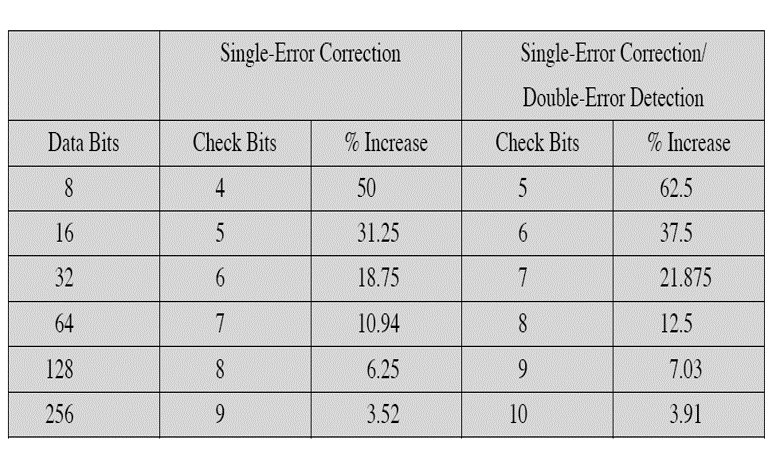
\includegraphics[width=3in]{pics/hamming.png}
  \caption[Procentul biților de paritate]{Procentul biților de paritate\protect\footnotemark}
  \label{fig:pic3}
\end{figure}
\footnotetext{© https://ocw.cs.pub.ro/courses/\_media/eim/curs/$03$.intro-radio.pdf}
\fi

Așa cum sugerează și figura~\ref{fig:pic3} procentul de overhead generat de acești biți de paritate atinge valori ideale (cât mai mici), pe măsură ce cantitatea de date este mai mare. Astfel, dacă nu este fezabil să folosim pentru doar 8 biți de date, generând un overhead de 50\% de date, folosirea pe o cantitate mai mare de date va genera un overhead foarte mic. De exemplu, pentru 256-502 biți de date se adaugă doar 9 biți de paritate, reprezentând undeva între 1-3\% din informația utilă. Numărul biților de paritate se calculează pe baza următoarei formule: $2^r > d + r + 1$, unde \textit{r} este numărul de biți redundanți, iar \textit{d} este numărul de biți de date. Noua informație se construiește prin punerea biților de paritate de pozițiile puteri ale lui 2, în timp ce restul pozițiilor sunt completate cu biții de date. Fiecare bit de paritate este calculat în felul următor:
\begin{itemize}
	\item parcurgând lista de biți de date se transformă indicele fiecărei poziții în binar
	\item fie $2^n$ poziția bitului de paritate
	\item se selectează biții de date a cărui indice are bitul \textit{n+1} cel mai puțin semnificativ setat în reprezentarea binară
	\item se aplică operația \textit{XOR} între biții selectați și valoarea se salvează pe poziția de paritate curentă
	\item astfel fiecare bit de date este inclus într-un set unic de biți de paritate
\end{itemize}

Respectând pașii descriși mai sus am creat noua informație formată atât din biți de date, cât și din biți de paritate. Simularea coruperii datelor este puțin diferită în acest context deoarece o singură corupere ar aduce întotdeauna un procentaj de 100\% al task-urilor primite corect. Atât datele simple, cât și datele extinse sunt grupate în clasa \textit{Data} și în funcție de parametrul de simulare (care poate permite sau nu utilizarea codurilor Hamming). În acest caz, coruperea are loc tot urmărind cele două scenarii prezentate în Subsecțiunea~\ref{simulareaCoruperii}, însă numărul biților corupți este ales random dintre 1,2 sau 3 pentru a nu permite corectarea biților la orice moment de timp. Pentru a putea afla poziția bitului corupt este nevoie de informația generată și de numărul biților de paritate. Se reia raționamentul de la generarea biților redundanți doar că toate calculele se realizează pe informația extinsă: biții de date și cei de paritate. Întervenind în calcule și valoarea biților de paritate rezultatul ar trebui să fie reprezentarea binară a lui 0 (în cazul în care nu s-a corupt niciun bit), altfel dacă rezultatul este diferit de 0, reprezentarea zecimală a lui reprezintă poziția bitului corupt. Modificând bitul cel mai nesemnificativ de pe acea poziție va rezulta data originală, dacă bitul de paritate al întregii date este schimbat. Dacă bitul de paritate pentru întreaga informație nu este schimbat și poziția rezultată nu este 0, înseamnă că s-au detectat mai mulți biți corupți și nu se poate realiza corecția.

\chapter{Detalii de implementare}	\label{detalii}

În acest capitol, vom detalia atât modul în care au fost implementate componentele introduse în capitolul~\ref{solutiaPropusa}, cât și limitarea altor abordări pe care le-am avut pe parcursul implementării. Secțiunea introductivă, \ref{introducere}, prezintă o sumarizare a implementării framework-ului MobEmu pentru a se putea înțelege interacțiunea pe care am avut-o cu acesta, respectiv modificările pe care le-am realizat în cadrul lui. 
Urmând ca, secțiunea \ref{algoritmi}, împreună cu toate subsecțiunile ei, să detalieze algoritmii necesari identificați și descriși în capitolul precedent.
 
\section{Descriere framework MobEmu} \label{introducere}
MobEmu~\cite{MobEmuArticle} este un framework folosit pentru parsarea unor trace-uri de mobilitate, pentru simularea unor algoritmi de rutare și diseminare a datelor, iar în final se generează statistici cu privire la caracteristicile rețelei (rata de succes, latență, numărul de contacte etc.). Principalele componente care se identifică sunt:  clasa \textit{Trace} și clasa \textit{Node}, care la rândul lor prezintă mai multe caracteristici precum: \textit{Context, Parser, Contact} pentru componenta \textit{Trace} și \textit{Altruism, Battery, Message, Topic, etc} pentru componenta \textit{Node}.

Componenta \textit{Trace} conține o listă de \textit{Contacte} ce deține informații necesare stabilirii unui istoric al contactelor, precum momentul de timp de început și sfârșit al contactului, dar și tipul contactului în funcție de tehnologia de detecție(e.g Bluetooth, WiFi). Pentru obținerea unui obiect de tip \textit{Trace} trebuie rulat un \textit{Parser}, o inferfață ce oferă următoarele informații: preferința nodului, conexiunile sociale (Facebook, Twitter) ale fiecărui nod, numărul de noduri din rețea și datele obiectului \textit{Trace} prin metodele: \textit{getContextData(), getSocialNetwork(), getNodesNumber(), getTraceData()}(are rost sa zic asta??). Această interfață are mai multe implementări în cadrul simulatorului, dintre care am utilizat clasa \textit{UPB} ce parsează datele unor trace-uri realizate în facultate în anii 2011 și 2012, și clasa \textit{HCMM} care este un generator de contacte utilizând un model sintetic, matematic ce simulează diferite comportamente ale nodurilor în funcție de anumite restricții impuse.

Un obiect de tip \textit{Node} conține toate informațiile necesare unui dispozitiv aflat într-o rețea oportunistă în care poate să ruleze algoritmi de rutare și diseminare a datelor. Principalele informații sunt legate de caracteristici interne precum id-ul care este unic, nivelul bateriei, lista propriilor mesaje, dar și cantitatea de memorie care este disponibilă pentru mesajele primite de la nodurile întâlnite (mesaje ce sunt destinate altor noduri). Această memorie reprezintă punctul central în cadrul implementării paradigmei store-carry-and-forward și cu cât este mai mare, cu atât cresc șansele la o rată de succes ridicată în cadrul rețelei. Alături de această memorie, se definește separat memoria mesajelor generate de fiecare nod în parte deoarece vor fi tratate diferit, nefiind șterse până la finalizarea respectivelor acțiuni. În timp ce, pentru memoria de date se implementează o politică de înlocuire, precum cea a memoriei cache, în momentul în care devine neîncăpătoare pentru acceptarea de noi mesaje. 
Informațiile deținute într-un obiect de tip \textit{Node} se continuă cu detalii despre contactele dintre noduri(noduri unice întâlnite, durata contactului cu un anumit nod într-o anumită perioadă), comunitatea locală detectată, cât și statistici cu privire la numărul de mesaje schimbate în rețea. 

Clasa \textit{Node} este o clasă abstractă și este extinsă de orice algoritm care vrea să aducă o nouă abordare în rutarea și diseminare oportunistă, implementând metoda abstractă \textit{onDataExchange()}. În continuare, vom prezenta pe scurt comportamentul simulatorului în momentul în care două noduri se întâlnesc, iar în următoarea secțiune se va detalia implementarea mecanismelor de consistență din cadrul paradigmei Drop Computing\cite{DC}. În momentul în care în urma parsării datelor dintr-un trace se identifică o conexiune validă între două noduri (contactul durează minim o anumită perioadă), se salvează referințe către nodul observator și nodul observat și în cazul unei noi conexiuni se apelează metoda \textit{exchangeData()}. Dacă un contact între aceleași două noduri nu este deja în progres, posibil în urma unor diferențe ale intervalelor de eșantionare ale fiecărui dispozitiv, se apelează metoda \textit{onDataExchange()}. Metoda primește ca parametrii nodul întâlnit, durata contactului și momentul de timp curent, urmând ca în implementarea ei să se regăsească toată logica referitoare la schimbul de informații. 

\section{Detalierea algoritmilor de realizare a consistenței}  \label{algoritmi}
Replicarea aceluiași task în mai multe noduri se realizează prin intermediul aceluiași obiect în Java, astfel nu se poate simula coruperea datelor în cadrul câmpului \textit{Data} din cadrul unui obiect de tipul \textit{Task}. În acest fel orice modificare adusă de un nod unui task ar fi fost resimțită în toate nodurile în care acesta a fost replicat chiar și înainte de a fi modificat. Prin urmare, se salvează în cadrul fiecărui obiect \textit{Task} un map în care sunt salvate toate locațiile în care este prezent fiecare task împreună cu valoarea datelor deținute de acele noduri.

Alături de map-ul care reține datele unui task, am folosit încă un map în cadrul clasei \textit{Task} care să facă legătura între id-ul nodului în care este prezent și executantul acelei versiuni, în cazul în care este vorba de un task completat. În momentul în care se interschimbă atât task-uri completate, cât și task-uri încă neexecutate, se salvează valoarea din map asociată id-ului nodului vizitat într-o nouă intrare în map ce are valoarea cheii egală cu id-ul noului nod posesor. În cazul task-urilor neexecutate nu se salvează id-ul executantului întrucât acesta încă nu există și se poate suprascrie o informație importantă deținută despre acel nod (map-ul dintre id-nod și id-executant poate conține o valoare pentru acel nod deoarece se poate ca acel nod să fi primit o versiune completată a aceluiași task, ulterior să o transfere mai departe și în cele din urmă să mai accepte și o versiune încă necompletată). Este foarte importantă identificarea corectă a executanților replicilor deoarece în urma depistării unei versiuni corupte trebuie identificat nodul executant și parcursă calea de la executant până la proprietar în vederea stabilirii nodurilor corupte. 

\subsection{Necesitatea adaugării timestamp-ului}
În clasa \textit{Task} se reține o listă cu toate căile parcurse de task de la proprietar, din momentul generării task-ului și până la momentul curent de timp. La rândul lor, căile sunt reprezentate printr-o listă de noduri pe care task-ul a parcurs-o în ordine. La început această listă este inițiată cu nodul proprietat, și ulterior se adaugă fiecare nod vizitat. În momentul în care un nod transmite un task completat sau necompletat nodului întâlnit și nu este îndeplinită condiția de familiariate cu acesta, se duplică calea existentă și se adaugă în lista de drumuri după ce se adaugă id-ul noului nod întâlnit. Acest lucru este necesar deoarece adăugarea unei noi căi se face căutând calea ce se termină cu id-ul nodului ce transferă informație, iar în situația descrisă anterior, task-ul încă mai este păstrat în memoria nodului și acesta poate să îl transfere și la viitoarele interacțiuni cu alte noduri. Adăugarea unui nod în această listă de căi se face întotdeauna prin generarea unei noi căi, copia celei deja existente, la care se adaugă noul nod. Această adăugare are loc în metoda \textit{onDataExchange()} indiferent de momentul de timp în care un task se schimbă (completat, neexecutat sau din nou la proprietar), iar pentru a șterge o anumită cale se apelează metoda separată \textit{deletePath()}(aceasta primește ca parametri lista de drumuri și id-ul nodului care nu mai poate disemina task-ul). Task-urile transferate sunt salvate într-o listă, iar în situația în care este îndeplinită condiția de familiaritate pe lângă ștergerea din memoria nodului în care au fost prezente, se șterg și căile pe care acestea au sosit până la respectivele noduri.

\begin{figure}[th]
\centering
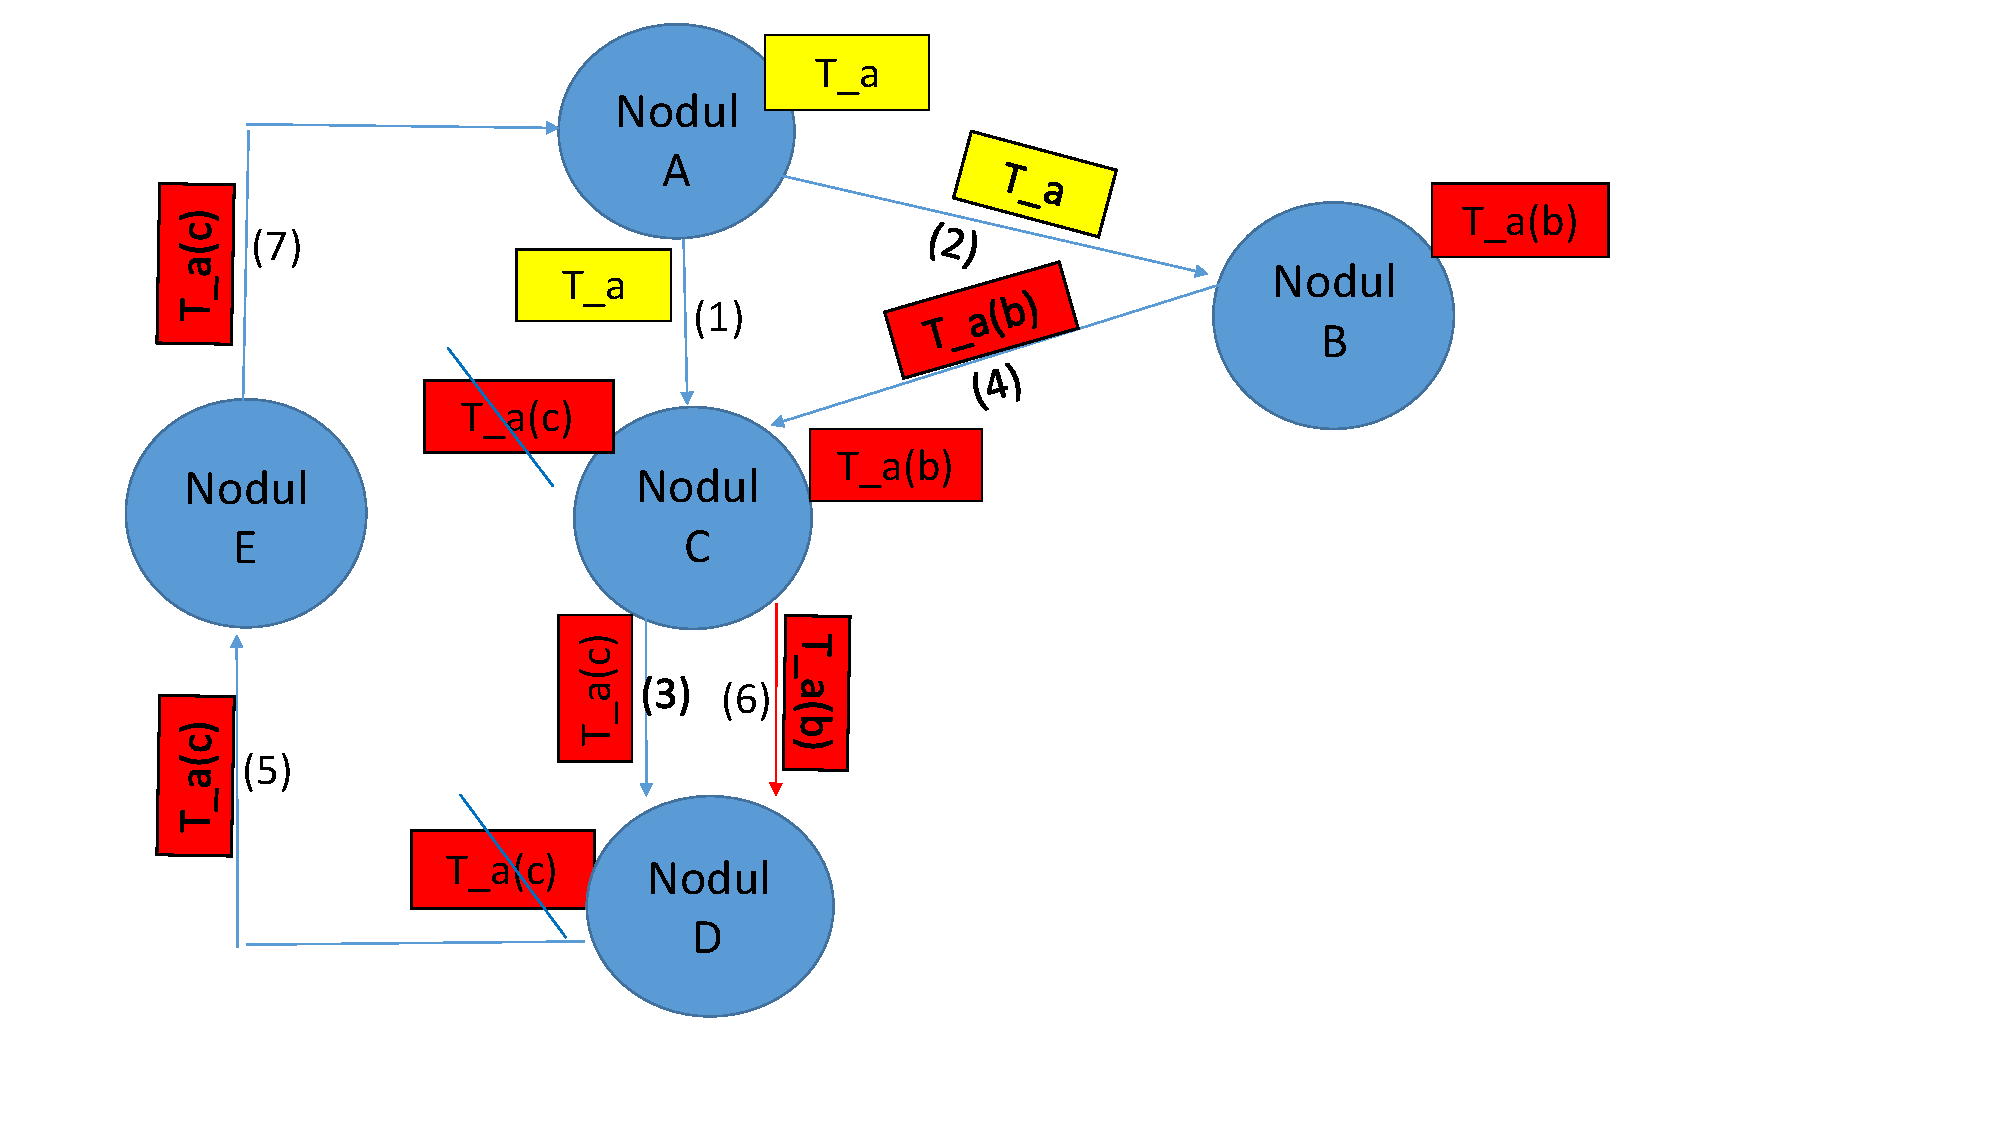
\includegraphics[width=4in]{pics/Timestamp.pdf}
  \caption[ca]{Necesitate timestamp}
  \label{fig:timestamp}
\end{figure}

Pentru a reține toate versiunile de task-uri care se trimit între aceleași două noduri se folosește încă un map în care cheile sunt reprezentate de valori de tipul \textit{SenderAndReceiver}, având ca valori \textit{List$<$ValueAndTime$>$}. Clasa \textit{SenderAndReceiver} are ca și caracteristici id-urile nodurilor emițător și receptor, iar în cadrul ei sunt suprascrise metodele \textit{hashcode()} și \textit{equals()} pentru a se putea accesa informația din map când se creează un nou obiect de tipul \textit{SenderAndReceiver} cu același emițător și receptor. Astfel, în momentul în care se parcurge calea pe care a ajuns un task completat la proprietar, trebuie verificate versiunile corecte de task-uri ce au fost schimbate de nodurile intermediare până la proprietar. Clasa \textit{ValueAndTime} reține informația task-ului transmis alături de momentul de timp la care a avut loc transmiterea, dar și de id-ul nodului care a executat acea versiune (dacă este vorba de o versiune neexecutată i se atribuie ca valoare un indicele nevalid -1).

În figura~\ref{fig:timestamp} este exemplificat un scenariu de transfer între noduri în care folosirea timestamp-ului este necesară pentru a lua deciziile corecte cu privire la nodurile rețelei. Fie nodul A proprietarului task-ului \textit{$T\_a$}, culoarea galbenă reprezintă faptul că task-ul nu este încă executat, în urma întâlnirilor cu nodurile B și C (la momentele de timp (1) și (2)) task-ul este transferat pentru a crește șansele de execuție. Să presupunem că nodul C execută task-ul \textit{$T\_a(c)$}, culoarea roșie arată că este vorba de un task executat și valoarea din paranteză indică nodul executant. După o perioadă de timp nodul C îl transferă nodului D (momentul (3)) și ulterior îl șterge din memoria proprie pentru că a întâlnit un nod pe care îl consideră de încredere. Între timp nodul B execută și el task-ul (\textit{$T\_a(b)$}) și îl corupe înainte de a-l transfera nodului C, nod cu care intră și contact și care îl acceptă deoarece nu îl mai deține în lista de task-uri completate. Ulterior, nodul D se întâlnește cu nodul E, care reușeste să-l transmită proprietarului, moment în care se începe verificarea drumului parcurs. Până la momentul de timp în care nodul E realizează o conexiune cu proprietarul task-ului, nodul C transferă versiunea coruptă și nodului D deoarece acesta șterge versiunea anterioară odată cu transferul la nodul E. În momentul în care se începe verificarea corectitudinii, se identifică drumul parcurs ca fiind $A->C->D->A$ și se începe verificarea datelor din fiecare nod. Verificând fiecare transfer dintre noduri, fără folosirea unei liste de versiuni cu timestamp-uri diferite, s-ar identifica între nodul C și D informație coruptă, valorile din map fiind suprascrise odată cu transferul de la momentul (6). Ținând cont că până la C task-ul nu a fost executat se trage concluzia că nodul C a corupt task-ul și se începe mecanismul de scădere pentru rating-ul nodului C, mecanism descris în Subsecțiunea~\ref{ratingSection}. Această concluzie nu este cea dorită deoarece nodul C este unul corect care nu a generat nicio corupere și un rating scăzut în mod greșit ar diminua șansele ca un task să fie propagat și executat cât mai repede prin rețea. Așadar, în implementarea propusă, se depistează existența mai multor versiuni de la nodul C către nodul D și se alege cea cu timestamp-ul mai mic față de versiunea transmisă de la nodul D la următorul nod din calea pe care a urmat-o task-ul până la proprietar. Astfel, se trage concluzia că versiunea transmisă a fost $T\_a(c)$, versiune care nu a fost coruptă și care a fost executată de nodul C, iar parcursul task-ului este cel de la momentele de timp ${(1),(3),(5),(7)}$.

\subsection{Detalierea mecanismelor de asigurare a consistenței}

Pentru o mai mare probabilitate de recepționare a unui task executat corect se așteaptă un număr variabil de versiuni, ce sunt salvate într-un map ale cărui chei sunt egale cu id-urile unice ale fiecărui task.
În metoda \textit{onDataExchange()}, în momentul în care un task completat ajunge la proprietar acesta nu este considerat încă executat ci este adăugat în lista de valori asociată id-ului task-ului pe care o găsim în map. Dacă map-ul nu conține încă cheia cu valoarea id-ului task-ului primit înseamnă că aceasta este prima versiune și se creează o nouă intrare în map. În cazul în care după primirea unei versiuni lista asociată task-ului are o lungime egală cu numărul dorit de versiuni se verifică informațiile primite folosindu-se funcția descrisă în Pseudocodul~\ref{alg:waitingVerification}.
\iftrue
\begin{algorithm}
\caption{Mecanismul de verificare a versiunilor primite}
\label{alg:waitingVerification}
\begin{algorithmic}[1]
\scriptsize
\State $L_{data}$ - lista versiunilor primite, $Task_{id}$ - id-ul task-ului primit, $T_{c}$ - numărul task-urilor corupte, $N_{versiuni}$ - numărul de versiuni așteptate, $Task_{data}$ - data nemodificată a task-ului curent

	\State fie $Majoritate$ $-$ procentul celor mai frecvente date din $L_{data}$
	\If {$Majoritate$ este egal cu $50\%$}
		\State mărește numărul versiunilor așteptate pentru task-ul $Task_{id}$ cu $1$
		\State ieșire din funcție
	\EndIf
	\ForAll {datele $D$ din lista $L_{data}$}
		\If {există coliziune între $D$ și $Task_{data}$} %?nu am explicat faptul ca aceasta data proprie a taskului nu se modifica
			\State crește $T_{c}$ cu 1
			\State resetează valoarea boolean-ului pentru corecția Hamming
		\EndIf
	\EndFor
	\If {$Majoritate$ $>$ $50\%$ și 2*$T_{c}$ $>$ $N_{versiuni}$}
		\State se acceptă o versiune coruptă
	\Else {} se acceptă o versiune consistentă
	\EndIf
	\State generare statistici în funcție de versiunile primite și de versiunile existente în rețea în acel moment de timp
\end{algorithmic}
\end{algorithm}    
\fi

În momentul în care se primesc toate versiunile așteptate se calculează o majoritate a datelor primite, adică procentajul informației cu cele mai multe apariții, aceea rezolvare a task-ului fiind cea care se va accepta de către proprietar. În cazul în care nu există o majoritate(liniile 2-5), adică sunt primite două sau mai multe versiuni diferite de același număr maxim de ori, nu se poate lua o decizie și se mai așteaptă o nouă versiune cu care să se formeze o majoritate (cu hamming se schimbă situația!!). Specificăm faptul că numărul de versiuni este o caracteristică a fiecărui task, astfel se crește numărul de așteptare al versiunilor doar pentru acel task, celelalte task-uri păstrând valoarea globală de așteptare. Parcurgând lista de informații primite se stabilește dacă există o diferență între datele proprii nealterate și datele primite (liniile 8-11) folosind funcția de hash descrisă în Subsecțiunea~\ref{hash}. Această funcție de verificare a coliziuniilor are un parametru de tipul \textit{MutableBoolean} care permite modificarea valorii aceluiași obiect din \textit{true} în \textit{false} și invers. Existența acestui parametru este utilă deoarece în situația în care se corectează folosind codul Hamming un bit acest lucru trebuie detectat și din exterior pentru a cunoaște faptul că un anumit nod a încercat coruperea înformației. În cazul în care majoritatea versiunilor primite au fost corupte (liniile 13-17) se salvează această informație într-un boolean și se trimite ca parametru funcției de generare a statisticilor. Această informație este necesară pentru a compara dacă acceptarea de informație coruptă a venit dintr-un număr majoritar sau minoritar de versiuni corupte existente în toată rețeaua, în acel moment.

Mecanismul de verificare al rating-ului nodurilor se desfășoară conform algoritmului detaliat în Pseudocodul~\ref{alg:ratingVerification}. Fiecare nod are un timer asociat caracteristicii de rating care se scade de fiecare dată când valoarea rating-ului nodului nu scade (în momentul în care scade ratingul acest timer este resetat la valoarea inițială). Acest timer oferă posibilitatea creșterii ratingului nodului după un anumit timp în care nu a mai generat nicio corupere. Nivelul de încredere al unui nod se acordă în funcție de valoarea rating-ului, iar scăderea acestuia la fiecare corupere conduce la un număr mare de noduri evitate. Creșterea rating-ului este benefică și ajută nodurile care generează întâmplător, în funcție de anumiți factori externi la momente depărtate de timp, coruperea datelor. Majoritatea task-urilor dintre momentele respective fiind executate și transportate fără nicio corupere. Evitarea acestor noduri conduce la scăderea ratei de succes a întregii rețele deoarece rezolvarea task-urilor nu se putea termina în timp util prin îmbinarea părților (subtask-urilor) provenite de la nodurile rețelei. Prin urmare, task-ul ajungea să fie executat folosind tot puterea de calcul a nodului proprietar, însă după un timp de așteptare pierdut. 
\begin{algorithm}
\caption{Mecanismul de verificare a ratingului nodurilor}
\label{alg:ratingVerification}
\begin{algorithmic}[1]
\scriptsize
\State $dcNodeId$ - id-ul nodului întâlnit, $NMap_R$ - map între id-urile nodurilor întâlnite de nodul curent și valorile rating-ului(în cazul primei întâlniri în acest map nu se află și nodul $dcNodeId$), $TMap_R$ - map între id nod și timer nod, $T_R$ - timer-ul inițial al ratingului, $Social$ - lista nodurilor ce compun rețeaua socială a nodului curent
	\If {$NMap_R$ conține nodul $dcNodeId$}
		\State scade timer-ul nodului cu 1 și îl pune în map-ul $TMap_R$
		\State fie $R_{value}$ valoarea cheii $dcNodeId$ conținută în $NMap_R$
		\State fie $T_{value}$ valoarea timer-ului din map-ul $TMap_R$ 
		\If {$R_{value}$ este între 50 și 100 și $T_{value}$ $<=$ 0}
				\State pune în $NMap_R$ valoarea minimă dintre 100 și $R_{value}$+20
				\State setează în $TMap_R$ pentru nodul întâlnit valoarea inițială a timer-ului $T_R$ 
		\EndIf
		\State $R_{value}$ - noua valoare din $NMap_R$
		\If {$R_{value}$ $>=$ 75.0}
			\State returnează adevărat
		\Else {} returnează fals
		\EndIf
	\EndIf
	\If {$Social$ conține $dcNodeId$}
		\State returnează adevărat
	\Else {} returnează fals
	\EndIf
\end{algorithmic}
\end{algorithm}

Schimbul de informații privind ratingul nodurilor întâlnite de fiecare dispozitiv mobil are loc în felul următor:
\begin{itemize}
	\item în momentul în care două noduri intră în contact transmit unul altuia lista proprie de ratinguri.
	\item dacă cele două noduri aflate în contact sunt în aceeași rețea socială, informațiile se schimbă astfel:
	\begin{itemize}
		\item se parcurge hashmap-ul de rating-uri ale nodului vizitat.
		\item dacă nodul curent deține în lista proprie ratingul acelui nod, se recalculează un rating nou făcând o medie aritmetică ponderată între cele două valori ( folosind o pondere de $60\%$ pentru valoarea proprie, respectiv $40\%$ pentru valoarea primită).
		\item dacă nodul curent nu deținea ratingul acelui nod, salvează valoarea primită având încredere în nodul din aceeași rețea socială.
	\end{itemize}
	\item dacă cele două noduri aflate în contact nu fac parte din aceeași rețea socială, informațiile se schimbă astfel:
		\begin{itemize}
			\item dacă nodul curent deține în lista proprie ratingul acelei nod, se recalculează un rating nou făcând o medie aritmetică ponderată între cele două valori (de data aceasta folosindu-se o pondere de $80\%$ pentru valoarea proprie, respectiv $20\%$ pentru valoarea primită).
			\item dacă nodul curent primește un rating pentru un nod necunoscut, nu îl salvează, așteptând o informație de la un nod familiar.
		\end{itemize}
	\item acest mecanism se aplică în momentul în care valoarea deținută pentru ratingul nodului întâlnit este mai mare ca 75.
\end{itemize}

Mecanismul de verificare a rating-ului~\ref{alg:ratingVerification} este apelat la fiecare interacțiune în funcția \textit{onDataExchange()} atât la schimbarea de task-uri completate, cât și la balansarea listelor de task-uri încă neexecutate. În situația în care funcția întoarce \textit{false} se trece la următorul nod întâlnit, nerealizându-se niciun schimb de informații. Funcția returnează \textit{false} dacă ratingul deținut pentru acel nod nu are o valoare cel putin egală cu 75 (ratingul 75 se obține în cazul unei singure coruperi) sau dacă nu sunt în aceeași rețea socială (liniile 16-18) și nu are o valoarea salvată pentru ratingul nodului întâlnit. Timerul destinat rating-ului fiecărui nod se scade la fiecare apel de funcție (linia 3) deoarece în cazul unei recalculări se resetează la valoarea inițială (linia 8). Acest timer dă posibilitatea nodurilor să își ridice nivelul rating-ului chiar dacă au generat la un moment dat coruperi, procesând însă, într-un timp setat, doar versiuni corecte. După expirarea timer-ului, dacă nodul are un nivel promițător (rating mai mare ca 50\%, mai mult de 2 coruperi succesive fiind considerate nejustificate) se crește valoarea rating-ului cu 20 și se resetează timerul (liniile 6-8). Se salvează în hashmap valoarea minimă dintre 100 și noua valoare deoarece nu se permite unui nod să își crească intenționat ratingul o perioadă, urmând ca mai apoi să corupă un număr mare de informații și să fie considerat de încredere atât timp cât ratingul nu a scăzut sub 75. 
 
Pentru a înțelege cât mai bine selectarea drumului real pe care îl parcurge un task de la generare și până ajunge executat la proprietar am adăugat în capitolul~\ref{anexe} algoritmul de selecție format din funcțiile ~\ref{alg:addNodeInPath} și ~\ref{alg:findMaxTimestamp}. Inițial, pentru salvarea drumului unui task, am folosit un graf orientat realizând o parcurgere BFS pentru a selecta drumul curent străbătut. Această abordare este detaliată în algoritmul~\ref{alg:historyOfTask}, în urma rulării descoperind multiplele posibilități de transfer între aceleași două noduri, algoritmul găsind mai multe căi până la nodul destinație. Astfel s-a observat necesitatea salvării tuturor transferurilor de task-uri împreună cu momentul de timp curent pentru a putea diferenția versiunile consistente de cele inconsistente, ceea ce conduce la aflarea nodurilor corupte.
% am trecut la abordarea cu timestamp și cu  
\chapter{Evaluare} \label{evaluare}

În acest capitol vom prezenta atât simulările în care am testat implementarea propusă, cât și analiza rezultatelor obținute în funcție de mai multe metrici pe care le vom prezenta ulterior.

Primul scenariu de mobilitate a unor dispozitive mobile a fost realizată folosind modelul HCMM~\cite{hcmm}, model ce simulează comportamentul și interacțiunile dintre mai multe noduri. Acest model include atât un comportament influențat de apartenența la o anumită rețea socială, cât și atracția asupra unor locații fizice specifice. Pentru acest scenariu, am creat următoarea simulare: 30 de noduri mobile, grupate în 5 comunități diferite, interacționează timp de 6 ore, 5 noduri dintre acestea fiind noduri călătoare (ele își pot schimba comunitatea inițială). Aria de desfășurare este de 1000 metri pătrați și viteza nodurilor este setată între 1.25 și 1.5 m/s, iar distanța până la care se poate realiza interacțiunea dintre 2 noduri este de 10 metri.

Alături de acest model de mobilitate sintetic am folosit și două trace-uri reale de mobilitate (\textit{UPB 2011~\cite{upb2011} și UPB 2012~\cite{upb2012}}) înregistrate în urma unor interacțiuni dintre noduri(dispozitive) reale. Trace-ul \textit{UPB 2011} este rezultatul unui experiment desfășurat în cadrul Universității Politehnica din București care cu ajutorul unei aplicații Android au înregistrat orice dispozitiv ce avea Bluetooth-ul activat. Datele pentru trace-ul \textit{UPB 2012} au fost înregistrate tot cu ajutorul unei aplicații Android, în același cadrul, având însă un număr mai mare de participanți (66 spre deosebire de 22 în cazul \textit{UPB 2011}). Alături de conexiunea Bluetooth, cel de-al doilea trace real, folosește și conexiunea Wi-Fi, înregistrând conexiunile atât cu celelalte dispozitive, cât și cu access point-urile wireless întâlnite. Conexiunea Wi-Fi oferă o mai bună stabilitatea, în schimb necesită un consum mai mare de baterie. Aplicația, rulând pe fundal, înregistrează și statistici referitoare la nivelul bateriei, la memoria disponibilă și la datele înregistrate de la sensori. Ambele trace-uri salvează într-o matrice conexiunile sociale dintre participanți, în timp ce în al doilea trace se extrag și interesele comune dintre aceștia, grupate pe categorii în urma analizării profilelor de Facebook.

Pentru a evalua implementarea propusă am propus trei metrici cu ajutorul cărora am luat măsurători în cazul mai multor scenarii de realizare a consistenței. Cele trei metrici sunt:
\begin{itemize}
	\item procentajul de task-uri corecte de ajung la proprietar executate de alte noduri din rețea.
	\item câte task-uri ajung executate de nodurile rețelei la proprietar (rezultat care variază în funcție de numărul de versiuni așteptate înainte de a lua o decizie).
	\item latența medie de procesare pentru fiecare task executat de alte noduri (timpul de la generare și până când proprietarul îl primește rezolvat).
\end{itemize}
Valorile acestor metrici sunt analizate atât cantitativ, cât și calitativ în următoarele situații:
În continuare, vom analiza rezultate obținute în următoarele situații:
\begin{itemize}
	\item simularea coruperii datelor, ținând cont de ambele scenarii descrise în subsecțiunea~\ref{simulareaCoruperii}, fără implicarea niciunui mecanism de realizare a consistenței.
	\item variația numărului de versiuni așteptate (3 sau 4, reamintind faptul că în cazul în care există două versiuni cu aceași frecvență se va mai aștepta o versiune pentru task-ul respectiv).
	\item folosirea sau absența mecanismului de rating (în cazul utilizării variind și valoarea rating-ului de referință).
	\item variația procentului de executanți diferiți în funcția de numărul versiunilor dorite.
	\item utilizarea codurilor de corecție Hamming (variind numărul de coruperi al aceluiași task).
\end{itemize}

Analizând cele trei metrici se poate observa cum pentru primele două ar trebui să se genereze valori mai ridicate, în urma mecanismelor de realizare a consistenței implementate (o valoare cât mai ridicată fiind de preferat în cadrul unui sistem perfect). În timp ce, în cazul ultimei metrici, o valoare cât mai apropiată de rezultatul înregistrat în urma rezolvării task-urilor folosind resurse proprii este de preferat. Această concluzie nu este însă perfect valabilă în toate cazurile în care paradigma Drop Computing se poate folosi, menționând aici posibilitatea ca rezolvarea unui task să necesite acces la Internet, în timp ce dispozitivul mobil nu poate realiza o conexiune la Internet. În acest scenariu utilizarea nodurilor întâlnite pentru rezolvarea propriilor task-uri poate fi realizată într-un timp mai scurt față de așteptarea unei eventuale conexiuni la Internet al nodului local.

Setul complet de grafice este format din 45 grafice  (3 trace-uri * 3 metrici * 5 scenarii), în fiecare dintre ele fiind calculată o metrică pentru fiecare din cele cinci situații prezentate mai sus. Valoarea metricii este dispusă pe axa \textit{Oy}, în timp ce pe axa \textit{Ox} se variază propabilitatea de corupere a task-urilor. Cele 5 scenarii, la rândul lor, au fost variate cu diferite valori ale parametrilor și au fost reunite pe seturi de scenarii și adăugate în cadrul aceluiași grafic. Din setul complet de grafice s-au selectat și analizat cele mai reprezentative în acest capitol, iar restul au fost grupate pe fiecare trace în parte și adăugate în capitolul Anexe~\ref{anexe}. Legenda fiecărui tabel este detaliată în tabelul~\ref{tab:scenarii}, fiecare grafic măsurând o metrică în urma celor 5 situații, prezentate mai sus, alături de diferite variații de parametrii.

\begin{figure}%
    \centering
    \subfloat[]{{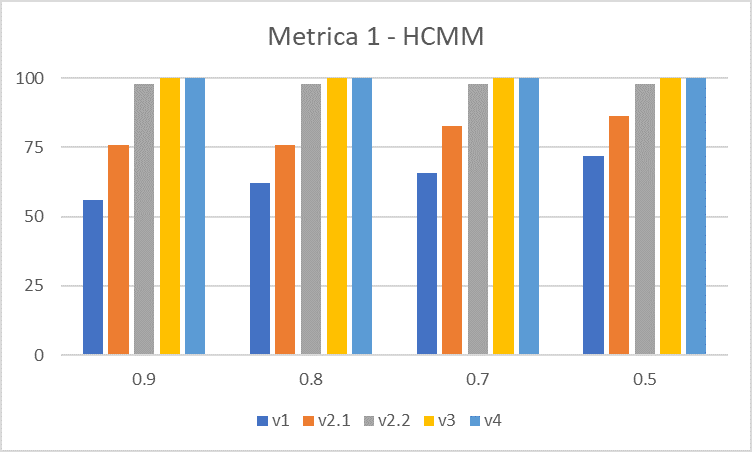
\includegraphics[width=7cm]{pics/graphics/grafic2.png} \label{fig:g1}}}%
    \qquad
    \subfloat[]{{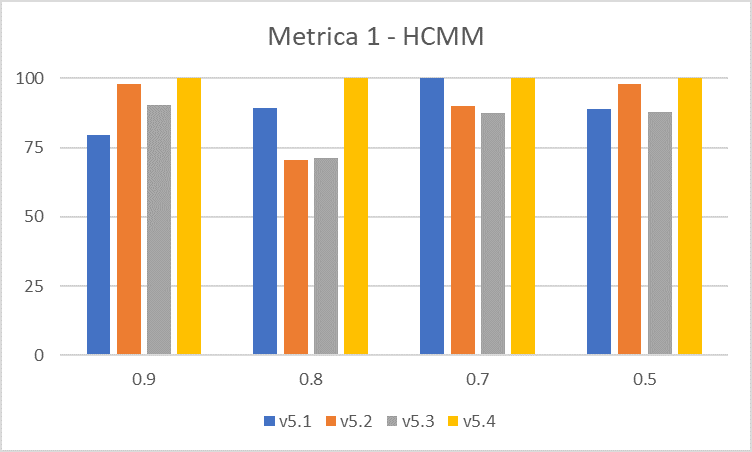
\includegraphics[width=7cm]{pics/graphics/grafic1.png} \label{fig:g2}}}%
    \caption{Procentajul/Variația task-urilor primite corect}%
    \label{fig:metric1HCMM}%
\end{figure}

Figura~\ref{fig:metric1HCMM} include două grafice ce măsoară procentajul de task-uri corect executate și transferate de nodurile rețelei către proprietar. Graficul~\ref{fig:g1} prezintă versiunea standard, \textit{v1}, al cărui procentaj este vizibil mai mic față de toate versiunile implementate în cadrul acestei lucrări. Graficul~\ref{fig:g2} reunește toate scenariile rulate folosind coduri de corecție și detecție Hamming, din care trebuie observat cum procentajul de task-uri primite corect nu crește simetric cu scăderea probabilității de corupere a nodurilor. Acest lucru se datorează faptului că în momentul coruperii se alege un număr random de coruperi dintre 1 și 3, existând posibilitatea ca proporția coruperilor cu mai mult de o poziție să fie mai ridicată chiar dacă per total se înregistrează mai puține coruperi. Cu toate acestea, se observă cum în toate scenariile prezentate în figura~\ref{fig:metric1HCMM} se înregistrează o pondere mai bună de rezultate corecte ca în versiunea existentă, \textit{v1}, aspect ce confirmă îmbunătățirile aduse prin intermediul acestei lucrări. Numărul de versiuni așteptate cu care s-a rulat scenariul cu mecanismul de rating a rezultat din urma analizei graficului~\ref{fig:versiuniRating}, prezentat în Anexe.

\begin{figure}%
    \centering
    \subfloat[]{{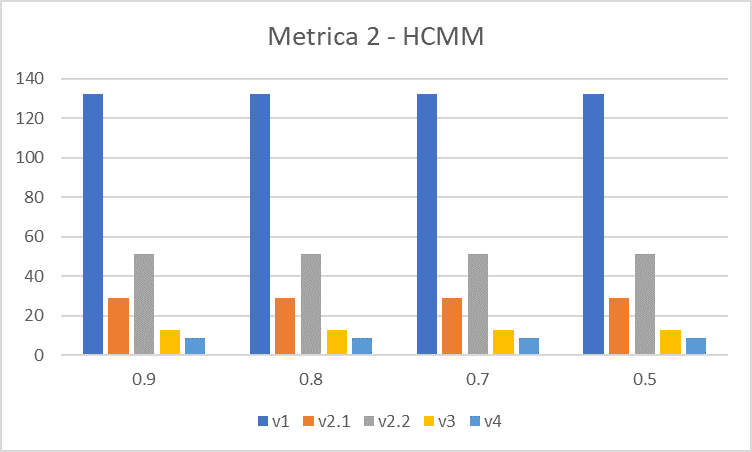
\includegraphics[width=7cm]{pics/graphics/grafic4.png} \label{fig:g3}}}%
    \qquad
    \subfloat[]{{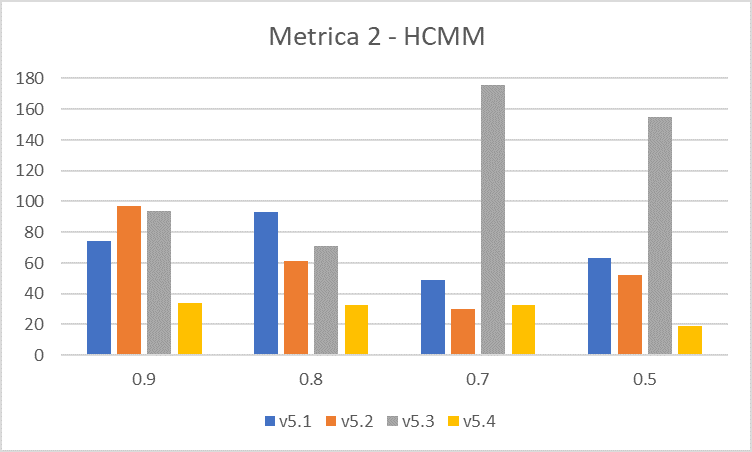
\includegraphics[width=7cm]{pics/graphics/grafic5.png} \label{fig:g4}}}%
    \caption{Numărul task-urilor executate în rețea}%
    \label{fig:metric2HCMM}%
\end{figure}

Valoarea mai scăzută a numărului de task-uri executate în rețea este confirmată prin graficele prezentate în figura~\ref{fig:metric2HCMM}. Așadar, această soluție oferă un grad de siguranță în ceea ce privește corectitudinea informațiilor cu costul unui număr mai mic de informații primite. Acest lucru se datorează atât filtrării nodurilor, cât și faptului că aceste simulări au fost făcute cu aceeași valoarea a timpului de așteptare al unui nod pentru orice task. Așadar, odată cu creșterea numărului de versiuni așteptate cresc și șansele ca un nod să-și execute propriile task-uri folosind doar propriile resurse.

\begin{figure}%
    \centering
    \subfloat[]{{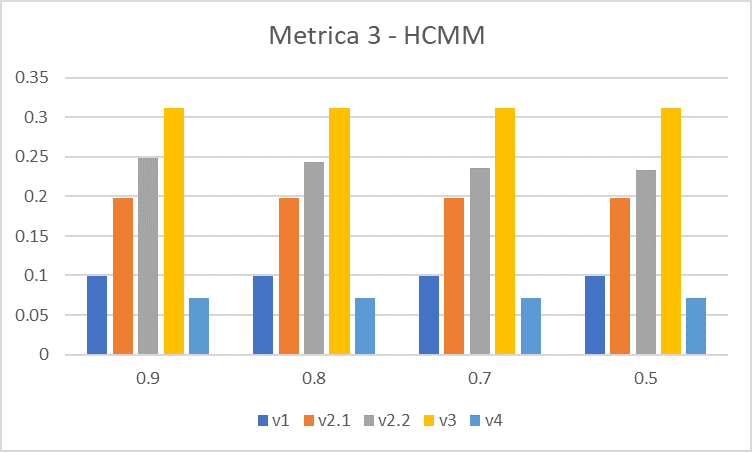
\includegraphics[width=7cm]{pics/graphics/grafic6.png} \label{fig:g5}}}%
    \qquad
    \subfloat[]{{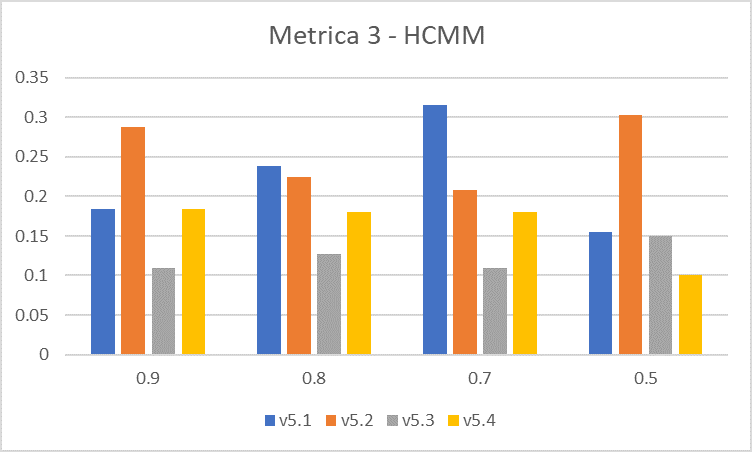
\includegraphics[width=7cm]{pics/graphics/grafic7.png} \label{fig:g6}}}%
    \caption{Numărul task-urilor executate în rețea}%
    \label{fig:metric3HCMM}%
\end{figure}
 
În figura~\ref{fig:metric3HCMM} se observă cum în principal se mărește latența medie de procesare pentru fiecare task primit executat din rețea, existând însă și cazuri în care valoarea ei este asemănătoare sau chiar mai mică (e.g v4, v5.3). Existența acestor situații arată faptul că întreaga rețea a fost acoperită eficient, task-urile fiind propagate prin noduri care într-adevăr au avut mai multe șanse de întâlnire cu proprietarul, în ciuda diminuării numărului de posibilități de transfer. Creșterea latenței de procesare fiind oarecum inevitabilă în momentul în care se așteaptă mai multe versiuni, însă se poate observa că procentul creșterii timpului nu este proportional cu procentul creșterii numărului de versiuni. (1 versiune - 0.09, 4 versiuni - 0.23). sa zic unitatea de masura

\begin{figure}%
    \centering
    \subfloat[]{{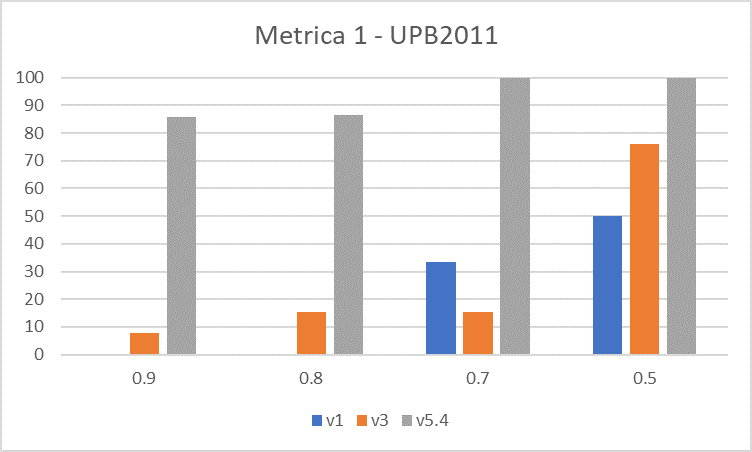
\includegraphics[width=7cm]{pics/graphics/grafic9.png} \label{fig:g7}}}%
    \qquad
    \subfloat[]{{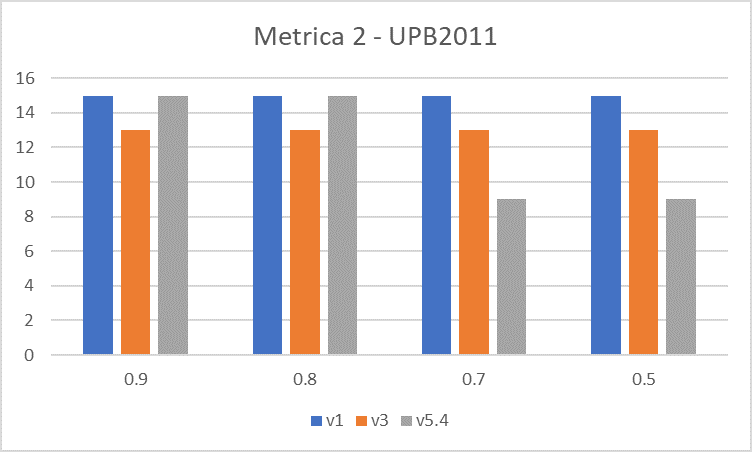
\includegraphics[width=7cm]{pics/graphics/grafic8.png} \label{fig:g8}}}%
    \caption{UPB2011}%
    \label{fig:metric12UPB2011}%
\end{figure}

Rezultatele obținute în urma simulării trace-ului UPB2011~\ref{upb2011} sunt evidențiate în graficele din figura~\ref{fig:metric12UPB2011}. Datorită faptului că în acestă simulare au fost folosite doar 20 de noduri, procentajul de noduri predispuse coruperii (30\%) este mai mare ca în cazul simulării HCMM (26\%), toate simulăriile fiind făcute cu presupunerea că 1 din 3 noduri pot corupe informații. Astfel, pentru o probabilitate mare de corupere, mai mică ca 0.9, s-a înregistrat un categoric 0\% procentaj de task-uri recepționate corect. Ținând cont de faptul că această simulare prezintă un număr mic de conexiuni între noduri, scenariile cu multiple versiuni de așteptare sau executanți diferiți nu au putut fi folosite. Cu toate acestea, utilizând mecanismul de rating și codurile de detecție Hamming se obține un procentaj cu până la 80\% mai ridicat de task-uri recepționate corect. Neconcordanța care apare în graficul~\ref{fig:g7}, la probabilitatea 0.7, procentajul de task-uri acceptate corupte, în urma aplicării mecanismului de rating, fiind mai scăzut față de cel obținut în versiunea standard este un caz izolat obținut datorită scăderii rating-ului unui nod care ulterior nu a mai realizat coruperi. Așadar, din cauza numărului mai mic de conexiuni între noduri, acesta nu reușește să își crească ratingul peste valoarea de referință, neavând suficiente oportunități de a transfera informațiile corecte pe care le deține.

Concluzionând, utilitatea acestei implementări se datorează procentului ridicat de task-uri corect recepționate de către proprietar, sugerând, astfel, o filtrare reușită de noduri predispuse coruperii ce a fost realizată datorită schimbului optimizat de mesaje utile. Principalele îmbunătățiri care se doresc a fi aduse acestei implementări sunt legate de scăderea latenței de procesare și de creșterea numărului de task-uri destinate altor noduri ce a ajung a fi executate în rețea. Aceste lucruri se doresc a fi realizate printr-o diferențiere și o propagare cât mai optimă a nodurilor care sunt predispuse coruperii, atât pentru a le evita, cât și pentru a crea un model al momentelor de timp în care aceste coruperi se realizează. Datorită numărului mare de grafice, rezultatele obținute în urma simulării trace-ului UPB2012~\ref{upb2012} sunt adăugate și analizate în Anexe, precizând că și ele respectă așteptările prezentate mai sus??. 

\chapter{Concluzii} \label{concluzii}
În această lucrare am propus și prezentat anumite mecanisme de consistență pentru schimbul de task-uri dintr-o paradigmă precum Drop Computing. Am oferit exemple de situații din viața reală în care această paradigmă are o bună aplicabilitate. Totodată, am subliniat și importanța primirii unor rezolvări corecte, nealterate în urma diferitelor pierderi sau coruperi de informații. În cadrul simulatorului MobEmu am adăugat numeroase statistici și modalități de descoperire a întregului istoric al schimbului de task-uri, de la nodurile care au participat la execuția lor și până la sursa coruperii.

Rezultatele obținute au arătat ca mecanismele implementate pot satisface, prin setarea restricțiilor potrivite, cerințele unei rețele în ceea ce privește nivelul de încredere dorit. De exemplu, în momentul în care informațiile care se schimbă sunt foarte importante și delicate, folosind mecanismul de rating se poate ajunge la procentaje de aproape $100\%$ privind acceptarea de task-uri executate corect. Acest mecanism prezintă o scădere a mesajelor și a task-urilor transmise prin rețeaua proporțională cu creșterea probabilității de corupere. Acest lucru se datorează faptului că multiple noduri vor ajunge la o valoarea mică a ratingului și vor fi considerate corupte, moment în care se va evita orice interacțiune cu ele. În schimb, folosirea sistemului de așteptare împreună cu diverse limitări în ceea ce privește calea pe care a venit, executantul acelei versiuni conduce la un număr mare de informații calculate cu ajutorul nodurilor cu care se interacționează. Scenariul descris anterior produce o anumită întârziere față de versiunea standard, dar prezintă o probabilitate mai bună de a accepta și folosi informații corecte, lucru care poate fi preferat în ciuda tuturor costurilor.

În prezent, paradigma Drop Computing este la stadiul de propunere, testând toată funcționalitatea cu ajutorul acestui framework, MobEmu, care prin simularea unor interacțiuni măsurate în viața reală încearcă să demonstreze utilitatea conceptului. Pe viitor ne dorim să îmbunătățim mecanismul de rating și să încercăm să găsim soluții pentru creșterea ratei de succes, în timp ce latența de procesare și overhead-ul să fie diminuate. O altă dezvoltare ulterioară vizează creșterea altruismului nodurilor prin integrarea unor mecanisme de recunoștință, ulterior fiecare nod să fie foarte interesat de rezolvarea și propagarea task-urilor vecinilor. Această recunoștință poate fi realizată atât financiar, cât și printr-o prioritizare diferită în rețea a task-urilor generate de nodurile altruiste.
Alături de codul de detecție și corecție Hamming, se dorește implementarea unui cod Reed-Solomon~\cite{reedSolomon}. Marele avantaj îl constituie posibilitatea de stabilire a overhead-ului, acest mecanism de corecție putând corecta un număr diferit de biți în funcție de numărul biților de paritate adăugați in mesaj. De asemenea, această implementare va putea rezista atât la o rafală de pierderi de un număr dorit de biți, cât și la același număr de biți corupți răspândiți aleator printre biții de date.

%Unul dintre ele este reprezentat de posibilitatea coruperii oricărei informații, chiar și informațiile statistice și rezultatele salvate tot în memoria nodului cu privire la ratingul celorlalte noduri întâlnite. In actuala implementarea nodurile corupte fiind descoperite pe baza unor noduri de incredere....

\chapter{Bibliografie} \label{bibliografie}

% Asa se specifica folosirea unui fisier cu referinte bibliografice:
\bibliographystyle{plain}
\bibliography{bibliografie}

%% Daca vreti ca o sectiune sa inceapa pe o pagina noua, puteti forta acest lucru cu comanda "\newpage", ca mai jos:
%\newpage

\chapter{Anexe} \label{anexe}
%\begin{algorithm}
%\caption{TEst}
%\label{}
\newlength\someheight
\setlength\someheight{3cm}
%\begin{adjustbox}{width=10in,height=\someheight,keepaspectratio}

\begin{lstlisting}[label={alg:historyOfTask},caption={Calea parcursă de un task până la destinație}]

public boolean historyOfTask(int source, int destination, LinkedList<LinkedList<Integer>> adjcent, List<Integer> intermidiateNodes) {

LinkedList<LinkedList<Integer>> paths = new LinkedList<>();	
LinkedList<Integer> firstPath = new LinkedList<Integer>();
firstPath.add(source);
paths.add(firstPath);
		
LinkedList<List<Integer>> pathFinder = new LinkedList<>();	
LinkedList<Integer> currentPath;
int currentVertex, elem;
Iterator<Integer> it;
boolean findPath = false, findDestination = false;
while (!paths.isEmpty() ) {
	findDestination = false;
	currentPath = paths.poll();
	currentVertex = currentPath.peekLast();
	if ( currentVertex == destination && !pathFinder.contains(currentPath)) {
		System.out.println("S-a gasit calea intre " + source + " si " + destination);
		printPath(currentPath);
		pathFinder.add(currentPath);
		findPath = true;
		findDestination = true;
	}
	if (!findDestination) {
		it = adjcent.get(currentVertex).iterator();		
		while(it.hasNext()){
			elem = it.next();
			if( !isVisited(elem, currentPath )){
				LinkedList<Integer> newPath = (LinkedList<Integer>) currentPath.clone();
				newPath.add(elem);
				paths.add(newPath);
			}
		}
	}
}
if(pathFinder.size() != 1 && findPath){
	System.out.println("S-au gasit mai multe cai se alege ultima, avand cele mai recente informatii");
	intermidiateNodes.addAll(pathFinder.get(pathFinder.size()-1).subList(1, pathFinder.get(pathFinder.size()-1).size()));
}	
return findPath;
}
\end{lstlisting}

\begin{lstlisting}[label={alg:addNodeInPath},caption={Aflarea căi potrivite}]

private void addNodeInPath(List<List<Integer>> paths, int idSender, int idReceiver, int taskId, Map<SenderAndReceiver, List<ValueAndTime>> newMap, int idExecutor, int idOwner, boolean completed) {
		
	boolean succes = false;
	LinkedList<Integer> list2 = null, list = null;
	int counter = 0;
	List<List<Integer>> foundedPaths = new LinkedList<>(); 
	Iterator<List<Integer>> it = paths.iterator();
	while ( it.hasNext() ) {
		list = (LinkedList<Integer>)it.next();
		if( list.peekLast() == idSender ) {
			succes = true;
			list2 = new LinkedList<Integer>(list);				
			foundedPaths.add(list2);
			counter++;
		}
	}			
	if(counter > 1) {
		list2 = findMaxTimestamp(foundedPaths, newMap, idExecutor, completed);
		System.out.println("Dintre toate caile " + foundedPaths + " s-a ales calea " + list2);
	}
	if(succes) {
		list2.add(idReceiver);
		paths.add(list2);
	}
}
\end{lstlisting}

\begin{lstlisting}[label={alg:findMaxTimestamp},caption={Aflarea versiunii potrivite}]
private LinkedList<Integer> findMaxTimestamp(List<List<Integer>> foundedPaths,
			Map<SenderAndReceiver, List<ValueAndTime>> newMap, int executorId, boolean completed) {
			
	long maxTime = 0, time;
	LinkedList<Integer> list2 = null;
	List<ValueAndTime> auxList;
	List<List<Integer>> testList = new LinkedList<>();
	if(!completed) {		
		/*taskul inca nu este executat inseamna ca voi alege versiunea care a venit cel mai tarziu*/
		for(List<Integer> list : foundedPaths ) {
			try {
				if(list.size() == 1)
					continue;
				auxList = newMap.get(new SenderAndReceiver(list.get(list.size()-2), list.get(list.size()-1)));		
				time = auxList.get(auxList.size()-1).getTimestamp(); 
				if(time > maxTime) {
					maxTime = time;
					list2 = (LinkedList<Integer>)list;
				}
			}catch(IndexOutOfBoundsException ex) {
				ex.printStackTrace();
			}
		}
	}else{	/*inseamna ca task-ul este executat*/
		for(List<Integer> list : foundedPaths) {
			if(list.contains(executorId))
				testList.add(list);
		}
		if(testList.size() == 1) {
			list2 = (LinkedList<Integer>)testList.get(0);
		}
		if(testList.size() > 1) {		
			/*pot contine mai multe executantul pentru ca taskul a mai putut trece si pe la nodul executant fara ca el sa fie completat*/
			int length = testList.size(), indexExecuter;
			ValueAndTime vat = null;
			for(int i = 0; i < length; i++) {	
				list2 = (LinkedList<Integer>)testList.get(length-i-1);
				indexExecuter = list2.lastIndexOf(executorId);
				if ( indexExecuter != list2.size()-1 ) {
					List<ValueAndTime> vatList = newMap.get(new SenderAndReceiver(list2.get(indexExecuter), list2.get(indexExecuter+1)));
					vat = vatList.get(vatList.size()-1);
				}	
			}
		}	
	}
	return list2;
	}
\end{lstlisting}

\begin{table}[th]\small\linespread{1}
\caption{Sumarizare scenariilor utilizate}
\label{tab:scenarii}
\begin{tabular}{l >{\raggedright\arraybackslash}p{8cm} >{\raggedright\arraybackslash}p{4cm}}
\textbf{Versiune} & \textbf{Situație} & \textbf{Observații} \\\hline
\textbf{v1} & Drop Computing standard &datele se pot corupe în ambele momente \\\hline
\textbf{v2.1} & v1 + 3 versiuni asteptate& \\\hline
\textbf{v2.2} & v1 + 4 versiuni asteptate &în cazul unei majorități de 50\% se mai așteaptă o versiune \\\hline
\textbf{v3} & v1 + 2 versiuni așteptate + sistemul de rating implementat &2 este numărul de versiuni cel mai potrivit, rezultat în urma analizei din tabelul  \\\hline
\textbf{v4} & v2.1 + cel mult 2 versiuni din 3 executate de același nod& \\\hline
\textbf{v5.1} & v2.1 + coduri de detecție și corecție Hamming& \\\hline
\textbf{v5.2} & v2.2 + coduri de detecție și corecție Hamming& \\\hline
\textbf{v5.3} & v1 + coduri de detecție și corecție Hamming& \\\hline
\textbf{v5.4} & v3 + coduri de detecție și corecție Hamming& sistemul de rating în acest caz a fost rulat fără a aștepta mai multe versiuni ale aceluiași task \\\hline
\textbf{m4} & numărul de versiuni corupte existe în toată rețeaua &\\
\hline
\end{tabular}
\end{table}

\begin{figure}[th]
\centering
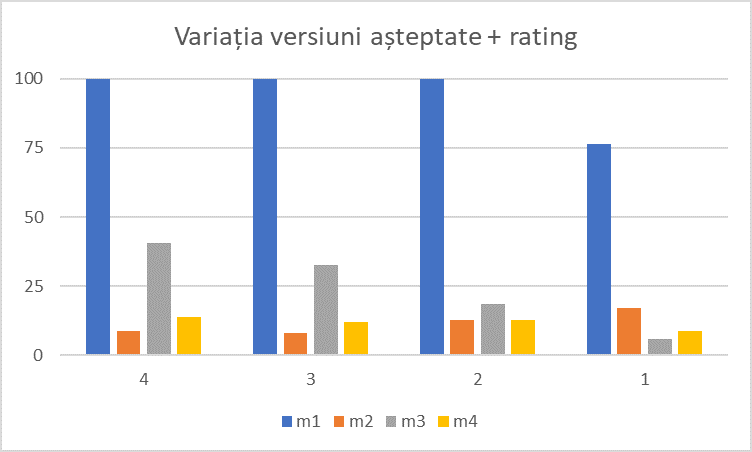
\includegraphics[width=4in]{pics/graphics/grafic3.png}
  \caption[]{Analiza mecanismului de rating}
  \label{fig:versiuniRating}
\end{figure}
În figura~\ref{fig:versiuniRating} s-au analizat toate cele 3 metrici descrise în lucrare, la care s-a mai adăugat metrica \textit{m4}, aceasta fiind descrisă în tabelul~\ref{tab:scenarii}. Fiecare metrică măsoară o altă unitate de măsură, de aceea am modificat valoarea latenței în minute pentru a avea valori dintr-un interval mai răstrâns. Pe axa Ox se variază numărul de versiuni așteptate și se observă cum cele mai bune valori se înregistrează la valoarea de 2 versiuni. În acest caz se înregistrează cea mai scăzută latență de procesare(m3) și cele mai multe task-uri executate în rețea(m2) dintre cele care prezintă un procentaj maxim de corectitudine(m1). 

\iftrue
\begin{figure}[th]
\centering
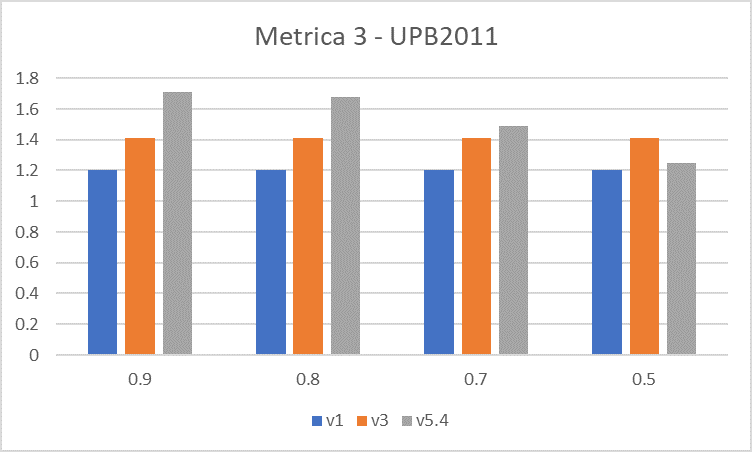
\includegraphics[width=4in]{pics/graphics/grafic10.png}
  \caption[]{Latența de procesare UPB2011}
  \label{grafic10}
\end{figure}
\fi

\iftrue
\begin{figure}[th]
\centering
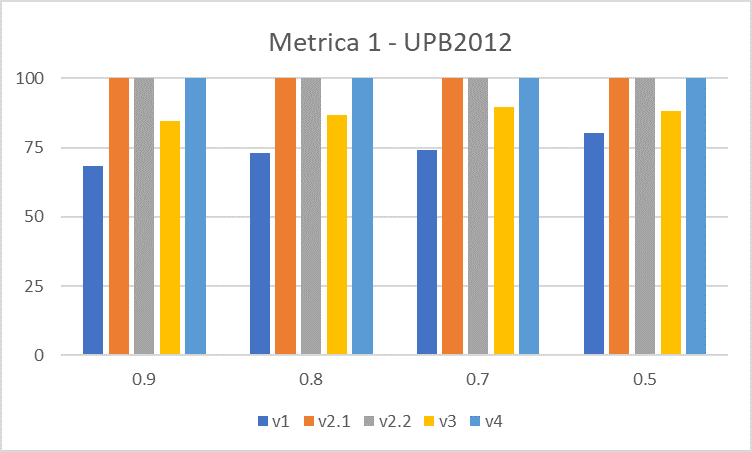
\includegraphics[width=4in]{pics/graphics/grafic11.png}
  \caption[]{Procentul task-urilor recepționate corect}
  \label{grafic11}
\end{figure}
\fi

\iftrue
\begin{figure}[th]
\centering
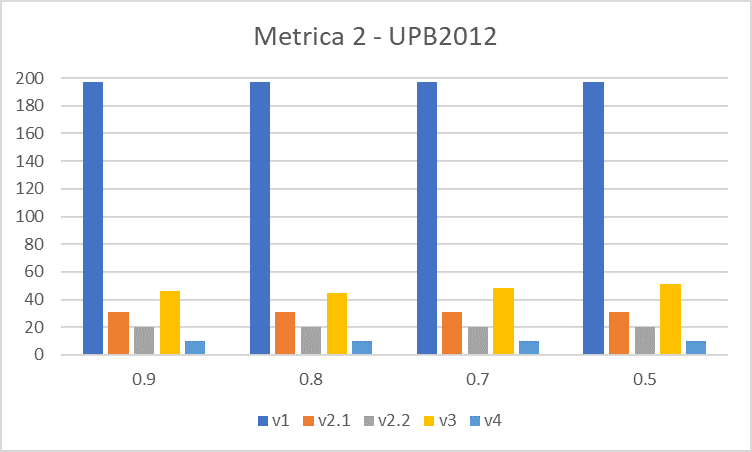
\includegraphics[width=4in]{pics/graphics/grafic12.png}
  \caption[]{Numărul task-urilor executate în rețea}
  \label{grafic12}
\end{figure}
\fi

\iftrue
\begin{figure}[th]
\centering
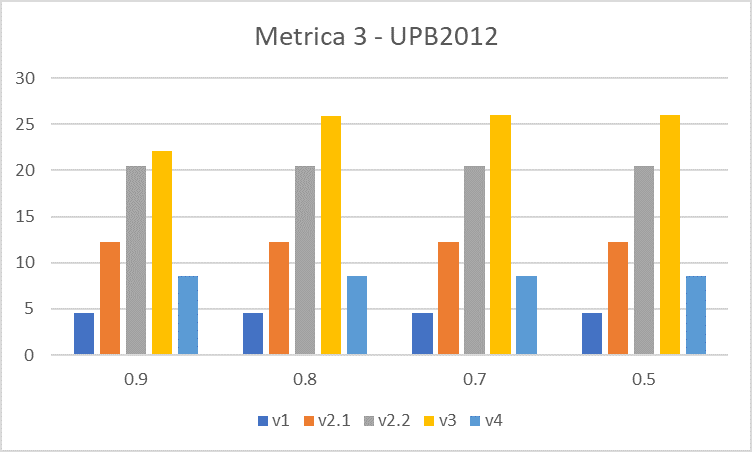
\includegraphics[width=3in]{pics/graphics/grafic13.png}
  \caption[]{Latența de procesare UPB2012}
  \label{grafic13}
\end{figure}
\fi
%\end{adjustbox}

\end{document}